\documentclass{article}
\usepackage{graphicx} % Required for inserting images
\usepackage[margin=1in]{geometry}
\usepackage{parskip}
\usepackage{amssymb}
\usepackage{amsmath}
\usepackage{amsthm}
\usepackage[table]{xcolor}
\usepackage{mathpartir}
\usepackage{stmaryrd}
\usepackage{hhline} 
\usepackage[colorlinks=true, linkcolor=blue, citecolor=blue]{hyperref}

\theoremstyle{definition}
\newtheorem{theorem}{Theorem}
\newtheorem{corollary}{Corollary}
\newtheorem{algorithm}{Algorithm}

\newcommand{\note}[1]{\textcolor{red}{#1}}
\newcommand{\xor}[0]{\textsf{xor}}
\newcommand{\blue}[1]{\textcolor{blue}{#1}}
\newcommand{\red}[1]{\textcolor{red}{#1}}
\definecolor{darkgreen}{rgb}{0,0.5,0}
\newcommand{\green}[1]{\textcolor{darkgreen}{#1}}
\newcommand{\purple}[1]{\textcolor{purple}{#1}}

\title{Automated Reasoning for Cryptographic Protocols}
\author{Rob Lorch}
\date{Spring 2026}

% \renewcommand{\familydefault}{\sfdefault}

\begin{document}

\begin{titlepage}
    \centering

    {\Large \textbf{Comprehensive Exam Report} \par}
    \vspace{0.5in}

    {\LARGE \textbf{Automated Reasoning for Cryptographic Protocols} \par}
    \vspace{.75in}

    {\large
    Submitted by\par
    \vspace{0.2in}
    \textbf{Robert Lorch}\par
    }
    \vspace{0.55in}

    {\large
    In partial fulfillment of the requirements for the Doctor of Philosophy\par
    Department of Computer Science\par
    The University of Iowa\par
    }
    \vspace{0.75in}

    {\large
    Examining Committee:\par
    \vspace{0.2in}
    Dr. Katherine Kosaian\par
    Dr. Garrett Morris\par
    Dr. Sourya Roy\par
    Dr. Cesare Tinelli\par
    }
    \vspace{1in}

    {\large
    April 23, 2026\par
    }

    \vfill
\end{titlepage}

\section{Abstract}

Security protocols are hard to prove correct. In fact, nailing down what correctness  
even means in the context of a security protocol is itself a nontrivial question, even before attempting a proof. 
The general difficulty of the problem has resulted in flawed ``proofs" of correctness, sometimes leading to real-world security impacts. 
Even worse, security concerns are often eschewed in favor of financial considerations, 
and so proofs are often not attempted in the first place.
In an ideal situation, one would like to define a security protocol, propose a security property, 
and have some automated tool either prove the protocol correct or return a concrete attack trace,
all with minimal human interaction. In this document, we describe various attempts to achieve this goal, 
while addressing a myriad of related questions along the way, 
largely focusing on \emph{expressivity} and \emph{tractability} of reasoning.

\section{Introduction}

% \note{Don't go over 35 pages + appendix; main text should be readable/followable without appendix}

% \note{Address Notes and Questions sections at the end}

% \note{Remember Cesare note about revealing the point in the abstract and intro; add to writing papers notes on docs too}

% \note{In general, take a pass and think about justifying correctness, or details that were elided (possibly 
% for lack of understanding)}

Security protocols are hard to get right. Examples abound of the discovery of inherent, 
design-level issues in security protocols only \textit{after} said protocols were designed, implemented, 
and in use \cite{lteinspector,5greasoner,ns_attack}. 
In this document, we argue that approaches based on \emph{formal methods} can help address these issues 
by aiding in the detection of security flaws at the project design level.
An often-cited example is the infamous Needham-Schroeder mutual authentication protocol \cite{needham_schroeder}, 
which we discuss in Section \ref{sec:sym-attacks}; its flaw was only discovered 17 years after the protocol 
was proposed with the help of formal tools \cite{ns_attack}.
Of course, there are also modern examples. A particularly relevant but tricky example 
is the 4G LTE/5G protocol stack \cite{4g_lte,5g}. 
The protocols are composed of various phases and layers, and they include the composition of cryptographic reasoning 
with non-cryptographic reasoning (e.g., linear integer arithmetic). 
Formal approaches to analyzing the 4G LTE and 5G protocol stacks have shown promise: 
they have resulted in the discovery of numerous design-level flaws, 
even when making the overly optimistic simplifying assumption that all cryptographic primitives 
are perfectly secure \cite{lteinspector,5greasoner,dolev_yao}. 
However, the state-of-the-art techniques \cite{lteinspector,5greasoner} still rely on manual interaction 
that requires expertise in \emph{two} separate formalisms, potentially suggesting an area for future improvement.

Late discovery of design-level problems has huge costs, financial and otherwise---it is estimated 
that problems discovered earlier at the \textit{design stage} (rather than the \textit{implementation stage}) 
of a software project
generally cost 5-30 times \emph{less} to address \cite{fm}. 
The current industry-standard method to detect software flaws is \textit{testing}. 
However, testing has limitations: $(i)$ it relies on the existence of a concrete implementation, 
$(ii)$ it can only prove the presence of bugs and never their absence, 
and $(iii)$ designing test cases that account for the wide range of possible adversarial influence is difficult. 
% {\begin{itemize}
%     \item Give motivation for reasoning about cryptography; Needham-Schroeder protocol
%     \item From Omar -- look at LTEInspector/5GReasoner work for motivation; real-world protocols have cryptographic components; one can forget about crypto but get spurious counterexamples; otherwise one has to integrate cryptographic reasoning. Even in cases where primitives are assumed secure there are real-world attacks. There are current approaches, model-based testing and abstraction/refinement to find these attacks. But they have downsides. But we need to take a step back and build a story based on details.
% \end{itemize}}
Therefore, to facilitate early detection of design flaws, we are interested in the formal verification of 
\textit{security protocols} with respect to \textit{security properties}, 
even under the influence of an \textit{adversary}, 
dubbed the \textit{security protocol verification problem} 
(where the notions of \textit{security protocol}, \textit{security property}, and \textit{adversary} will be elaborated later). 
We are particularly interested in \emph{(semi-)automated approaches} to addressing the 
security protocol verification problem, keeping in mind two core accompanying concerns,
\emph{expressivity} and \emph{tractability}:
approaches must be \emph{expressive enough} to model modern protocol features such as cryptographic primitives with 
algebraic properties (e.g. exclusive or), arithmetic constraints, and non-trivial control flow, 
while still remaining \emph{tractable enough} to produce proofs or counterexamples with minimal human interaction. 

\textbf{Scope.} This document gives an overview of the formal verification of software systems with cryptographic components. 
However, we give special focus to verifying \emph{cryptographic protocols} rather than \emph{cryptographic primitives} 
(e.g., encryption functions, hash functions), as well as the \emph{symbolic threat model}, 
which defines a set of adversary capabilities amenable to automation. 
Further, we will discuss implemented tools, but with a focus on two that dominate modern 
cryptographic protocol verification, Tamarin \cite{tamarin} and ProVerif \cite{proverif}. 

\textbf{Roadmap.} We will first discuss relevant background information relating to cryptography 
and cryptographic protocol verification, followed by an overview of typical security properties. 
With this context in mind, we define the symbolic threat model and outline approaches to formalizing 
protocols and properties in this threat model. Then, we discuss the mechanization and automation of reasoning, 
along with some of the major challenges (generally regarding expressivity). 
Next, we discuss metatheoretic results in the symbolic model 
that help address these challenges and make automated reasoning more tractable. 
Finally, we conclude with a discussion of open problems in the area.

\section{Security Background}\label{sec:crypto-background}
We start with an overview of standard cryptography-related concepts in computer security.
\subsection{Cryptography}
% The field of cryptography was somewhat ad hoc until recently (i.e., the 20th century). 
Cryptography was largely ad hoc until the mid-20th century, 
with a rigorous foundation beginning with Claude Shannon's 1949 work on information theory \cite{shannon} and modern 
cryptography emerging in the 1970s \cite{diffiehellman,rsa}.
Before the mid-20th century, cryptography largely centered around the study of \textit{ciphers}, 
which are methods to obscure a secret message being exchanged between two parties such that only the intended recipient, 
and not an eavesdropper, can recover the original message. 
Two famous ciphers are \textit{Caesar's cipher} \cite{textbook} and \textit{Vigenère's cipher} \cite{textbook}, 
which are widely discussed in cryptography textbooks (e.g., \cite{textbook}). 
Historically, ciphers were invented and used until they were cracked. 
If nobody was yet to crack a cipher, then it was considered secure.

In the ad hoc world, the only protection from malicious actors is the faith that they cannot crack your cipher. 
However, one would like to know that a cipher is \textit{provably} secure; 
that is, that it is accompanied with a proof that it is impossible to crack.
To achieve this goal, more rigorous definitions of security are required. 
We give an overview of mathematical definitions in the setting of \textit{symmetric-key cryptography} 
where a single shared key is used for both encrypting and decrypting messages; 
these concepts can naturally be extended to more complicated settings.

\textbf{Symmetric key encryption scheme.} 
Consider a set of messages $\mathcal{M}$, a set of ciphertexts $\mathcal{C}$, and a set of keys $\mathcal{K}$. 
Typically $\mathcal{M} = \mathcal{C} = \{0, 1\}^*$ and $\mathcal{K} = \{0,1\}^\lambda$ 
for a fixed security parameter $\lambda \in \mathbb{Z}^+$. 
Each \textit{plain text} $p \in \mathcal{M}$ intuitively represents a message to be shared, 
each \emph{ciphertext} $c \in \mathcal{C}$ represents an obscured plain text, 
and each \emph{key} $k \in \mathcal{K}$ can be used to help generate ciphertexts from plain texts. 
A \emph{symmetric-key encryption scheme} is a triple $(\mathsf{Gen}, \mathsf{Enc}, \mathsf{Dec})$ 
comprised of three functions  
$$\textsf{Gen} : \mathbb{N} \rightarrow \mathcal{K}, \textsf{Enc} : \mathcal{M} \times \mathcal{K} \rightarrow \mathcal{C}, 
\text{ and }\textsf{Dec} : \mathcal{C} \times \mathcal{K} \rightarrow \mathcal{M},$$
where $\textsf{Gen}(\lambda)$ probabilistically samples a key of length $\lambda$ from 
$\mathcal{K}$, and \textsf{Enc} and \textsf{Dec} denote encryption and decryption as expected. 
We require that 
$$\forall m \in \mathcal{M}, k \in \mathcal{K}.\;\mathsf{Dec}(\mathsf{Enc}(m, k), k) = m$$ 
Intuitively, decrypting a ciphertext using the same key used to encrypt it yields the underlying plain text.

\textbf{Kerckhoff's principle.} \textit{Kerckhoff's principle} states that the security of a scheme 
should only rely on the secrecy of keys and not of  algorithms (in this case, \textsf{Gen}, \textsf{Enc}, and \textsf{Dec}). 
There are four major arguments in favor of this principle: 
(1) it is easier to keep a key secret than an entire encryption scheme, especially for large organizations; 
(2) it is easier to replace a key than an encryption scheme if information is leaked; 
(3) keeping one (or a small set) of encryption schemes is more practical 
for wide-scale deployment of applications with cryptographic algorithms; 
(4) standardization of cryptographic schemes lends itself to public scrutiny, including attempts at formal verification. 
With Kerckhoff's principle, security becomes a problem that is amenable to mathematical analysis.

\textbf{Perfect secrecy.} With Kerckhoff's principle in mind, 
how does one determine when a symmetric key encryption scheme is secure? 
The gold standard is \textit{perfect secrecy}---the requirement is that for all probability distributions 
over $\mathcal{M}$, all $m \in \mathcal{M}$, and all $c \in \mathcal{C}$ such that $\text{Pr}[C=c] > 0$, 
$$\text{Pr}[M=m \mid C=c] = \text{Pr}[M=m].$$ 
Here, $Pr[M=m]$ denotes the probability that random variable $M$ (denoting the plain text) equals $m$
(a particular plain text), i.e., the probability that the sender sent message $m$ (and analogously for $Pr[C=c]$).
The bar $|$ denotes conditional probability.
Intuitively, this means that if an adversary observes a ciphertext $c$, 
it reveals no information about the value of its plain text $m$. 

Perfectly secret encryption schemes have an important property.

\begin{theorem}
For any perfectly secret encryption scheme, $|\mathcal{K}| \geq |\mathcal{M}|$ (with $|.|$ denoting cardinality).
\end{theorem}

However, two results follow.

\begin{corollary}\label{cor:ps}
If the length of $k$ is equal to $\lambda$ for all $k \in \mathcal{K}$ and $M = \{0,1\}^n$ for some $n$, 
then for any perfectly secret encryption scheme, $\lambda \geq n$. 
\end{corollary}

\begin{corollary}\label{cor:ps_2}
Using the same key to encrypt two distinct plain texts violates perfect secrecy.
\end{corollary}

 From Corollary \ref{cor:ps} and Corollary \ref{cor:ps_2}, 
 keys must be long (at least as long as the messages to send) and can never be reused. 
 From these results, in practice, perfect secrecy is often too strong of a requirement. 
 So, often times we settle for a weaker notion of security, with a common example being \textit{IND-CPA security}.

\textbf{IND-CPA security.} \textit{IND-CPA security} (\textbf{i}ndistinguishability under 
\textbf{c}hosen \textbf{p}laintext \textbf{a}ttack) is defined in terms of a game between a 
\textit{challenger} and an \textit{adversary}, where the scheme is deemed secure if the adversary 
can win the game with probability only negligibly larger than random chance. 
The game proceeds as follows (where $\xleftarrow{\$}$ denotes sampling from a probability distribution).

\begin{enumerate}
    \item $k \xleftarrow{\$} \mathsf{Gen}(1^\lambda)$
    \item The adversary is given knowledge of $\lambda$ and oracle access to $\mathsf{Enc}(., k)$
    \item The adversary chooses two messages $m_1$
 and $m_2$ such that $|m_1| = |m_2|$ (with $|.|$ denoting string length)
    \item $b \xleftarrow{\$} \{0, 1\}$ uniformly
    \item $c \xleftarrow{\$} \mathsf{Enc(m_b,k)}$
    \item Adversary is given $c$ and retains oracle access to $\mathsf{Enc}(., k)$
    \item Adversary outputs $b'$ and wins if $b' = b$
 \end{enumerate}
 Intuitively, the adversary generates two messages $m_1$ and $m_2$, one of them is encrypted at random, 
 and the adversary tries to guess which one. The scheme is secure if, for all probabilistic polynomial time (PPT) adversaries, 
 $\text{Pr}[\text{Adversary wins game}] \leq \frac{1}{2} + \textsf{negl}(\lambda)$, where $\textsf{negl}$ 
 is some negligible function.

 \subsection{Other Cryptosystem Preliminaries}
 \textbf{Types of keys and compromises.} 
 There are different types of cryptographic keys---\emph{long-term keys} are keys meant to be used across sessions, 
 while \emph{session keys} are keys only used in a single session. 
 A \emph{key compromise} is a scenario where the adversary has gained knowledge of some secret key, 
 and a \emph{principal compromise} is a scenario where the adversary controls one of the honest participants.
 

\textbf{Asymmetric key crypto.} Under \emph{asymmetric key cryptography}, 
every principal has a \textit{public key} and a \textit{secret key}. 
The public key is publicly known, 
while the secret key is only known to the principal who owns it. 
If $A$ (asymmetrically) encrypts $m$ with $B$'s public key, 
then it is computationally infeasible to recover $m$ without knowledge of $B$'s private key. 
Additionally, $A$ can \emph{digitally sign} message $m$ with $A$'s private key, 
producing a \emph{digital signature} which can be \emph{verified} using $A$'s public key. 
Here, it is computationally infeasible to produce a signature of a message $m$ 
that will pass verification with $A$'s public key without knowledge of $A$'s private key.
 Note that a digital signature is meant to guarantee authenticity, and an asymmetric encryption is meant to guarantee secrecy.

\textbf{Cryptographically secure hashes.} A \textit{cryptographically secure hash function} \textsf{h} has two properties: 
\begin{enumerate}
\itemsep-.5em
\item It is computationally infeasible to invert (called \textit{one-wayness}). 
\item It is computationally infeasible to find distinct $x$ and $x'$ such that $\textsf{h}(x) = \textsf{h}(x')$ (called \textit{(strong) collision resistance}).
\end{enumerate}

\textbf{XOR and DH exponentiation.} 
There are other cryptographic primitives in addition to the standard encryption and decryption.
 \emph{Exclusive or} is often used, as computing the (bitwise) exclusive or of a message with random bits produces 
 an output that is indistinguishable from random bits (in fact, it satisfies perfect secrecy).
Another common primitive is \emph{Diffie--Hellman exponentiation}. 
In this setting, principals operate in a cyclic group $G$ generated by an element $g$. 
Given a secret exponent $x$, the value $g^x$ can be computed efficiently, 
but recovering $x$ from $g^x$ is assumed to be computationally infeasible 
(if not, then the group is not suitable for Diffie--Hellman exponentiation).

\subsection{Cryptographic protocols}

A \emph{cryptographic protocol} is a standardized procedure followed by a group of parties communicating remotely 
over an insecure network channel in order to accomplish some goal, 
composing cryptographic primitives in an attempt to maintain a specified set of security properties. 
Each participant in the protocol description is called a \emph{role}, 
and each concrete participant of a particular protocol instance is called a \emph{principal} 
(each role can be instantiated by various principals). 
An \emph{honest participant} follows the protocol description, 
while the \emph{adversary} (also called the \emph{intruder} or \emph{attacker}) 
attempts to undermine the security guarantees of the protocol and can perform any action 
that is allowed according to a given \emph{threat model} 
(i.e., description of attacker capabilities).  
A \emph{session} is a single logical instance of a protocol, and a protocol \emph{trace} 
is a log of events associated with the execution of a protocol, possibly containing multiple sessions.
Each \emph{event} records a protocol action that took place, along with the relevant data items involved 
(e.g., the event \textsf{Secret}$(A, n_A)$ denotes that nonce $n_A$ was marked as secret by principal $A$).


\section{Cryptographic Primitive and Protocol Verification Background}
While \textit{cryptography} is a mathematical field, one might wonder how to mechanize reasoning 
about cryptographic systems. To do this, approaches must address the fundamental tradeoff between the 
\textit{level of automation provided by the approach} and the 
\textit{degree to which the approach respects mathematical cryptography}.

\subsection{General preliminaries}
We use $\rightarrow^*$ to denote the reflexive-transitive closure of binary relation $\rightarrow$. 
We use $\mathcal{P}(S)$ to denote the power set of set $S$. 
Notation $f \circ g$ denotes function composition of the form $g(f(x))$ for input $x$ 
(note that we evaluate $f$ first). 
A term $t$ is \textit{ground} if it does not contain variables. 
We use $\{x \mapsto M\}$ to denote the substitution of term $M$ for variable $x$, 
and we use postfix notation to denote the application of (the homomorphic extension of) a substitution 
to term $t$ (e.g., $t\{x \mapsto M\}$). 
We use notation $t[x_1, \dots, x_n]$ to denote that term $t$ has free variables $x_1$ through $x_n$, 
and $\mathit{fv}(t)$ to denote the free variables of term $t$. 
In discussions relating to $\pi$-calculus, we also use the prior two notations for processes (rather than terms). 
We use $\triangleq$ to denote ``equal by definition," 
and we use $f[x \mapsto y]$ to denote the function 
that maps $x$ to $y$ and otherwise agrees with $f$. 
Further preliminaries for more specific notation will be introduced later in the report, 
closer to where the notation is used. 

\subsection{Threat models} Approaches to verification can be classified based on the \textit{threat model}, 
i.e., the characterization of the adversary's capabilities as well as the security properties to prove. 
Approaches can generally be split into two camps, 
the \textit{computational model} and \textit{symbolic model}. 
Additionally, there a middle ground called the \textit{computationally complete symbolic attacker (CCSA) model}.

In the \textit{computational model} \cite{computational_model}, the semantics closely align with the mathematical formalism 
described in Section \ref{sec:crypto-background}---adversaries are PPT Turing machines, 
functions map bit strings to bit strings, 
and security properties are defined in terms of games and probabilities. 
The computational model will be discussed further in Section \ref{sec:computational-model}.

The \textit{symbolic threat model} \cite{dolev_yao} is characterized by the assumption that all cryptographic primitives 
are perfectly secure. In addition, security properties are reframed (and often weakened) 
to avoid reasoning about probabilities or games. 
All together, the symbolic model represents a generally weaker notion of security. 
However, it lends itself to automation and usability, and it is still strong enough to find many issues in practice. 
The symbolic model will be discussed in depth in Section \ref{sec:sym-threat-model}.

In the \textit{CCSA model} \cite{ccsa}, the set of adversarial capabilities is overapproximated 
(compared to the computational model), and the security property is strengthened. 
The approximations lend themselves to automation without weakening the notion of security as in the symbolic model. 
However, the approach may report spurious attacks which are not always straightforward to address. 
Further discussion of the CCSA model is outside the scope of this report. 

\subsection{Primitive vs protocol verification} 
The computational model can be used both to verify \textit{implementations of cryptographic primitives} as well as 
\textit{cryptographic protocols}, which can be viewed as the composition of cryptographic primitives in various ways.
However, the symbolic model (and CCSA model) focus solely on the verification of cryptographic protocols, 
where the properties of cryptographic primitives are axiomatized.
If primitives are assumed to be perfectly secure (as in the symbolic model), 
one might assume that their composition must also be secure (barring obvious problems, 
like directly exposing secret keys on a public channel). 
However, it is easy to compose even idealized primitives in a non-obviously insecure way. 

Consider a tiny protocol with a single step, $A \rightarrow B: \langle \textsf{sr\_enc}(m, k, \textit{IV}), \textsf{h}(m) \rangle$. 
This denotes that role $A$ sends to role $B$ a message with two components, 
the first of which is the symmetric randomized encryption of message $m$ with key $k$ and 
\emph{initialization vector} \emph{IV} (essentially, a random value), 
and the second of which is the hash of message $m$. This protocol intends to accomplish the following goals:
\begin{itemize}
    \item[] Assume $\mathit{IV}$ is fresh and $k$ is preshared between $A$ and $B$.
    \item[(1)] Guarantee secrecy of message $m$ through symmetric randomized encryption with 
    initialization vector \textit{IV}.
    \item[(2)] Guarantee \emph{integrity} of message $m$ (i.e., that $m$ was not modified in flight) 
    with cryptographically secure hash function $\mathsf{h}$.
\end{itemize}

For goal (1), idealized random encryption has stronger secrecy guarantees compared to deterministic (non-randomized) encryption, 
since encrypting the same message $m$ twice (with different $\textit{IV}$s) will yield distinct ciphertexts.
To reap this benefit, each encryption must use a distinct \emph{IV}, hence the assumption that \emph{IV} is fresh.
Further, for goal (2), the recipient can check that the message was not modified in flight by verifying 
that the hash of the plain text (after decrypting) matches the hash sent by $A$. 
However, composing the primitives in this way is insecure---since the hash function is deterministic, 
the adversary can count the number of times a given message is sent. 
While this does not directly leak the plain text, it is still a form of information leakage 
that randomized encryption is supposed to combat.

\subsection{Computational Model Verification}\label{sec:computational-model}
One can encode encryption schemes, security properties, and proofs in an interactive theorem prover (ITP) 
such as Lean \cite{lean} or Isabelle \cite{isabelle}. 
There also exist ITPs and frameworks that are designed with computational model proofs in mind 
(involving cryptographic games and probability distributions) 
such as EasyCrypt \cite{easycrypt} and CryptHOL \cite{crypthol}. 

Because the computational model directly captures mathematical cryptography, 
it can be considered a gold standard for verification.

While computational model tools can provide some level of automation, proofs are largely interactive. 
This report focuses on the verification of cryptographic protocols in the symbolic model, 
which attempts to give more automation (and hence further discussion of the computational model is out of scope).


\section{Security Properties}\label{sec:security-properties}

Here, we give an intuitive overview of common security properties to prove or falsify. 
More precise encodings are deferred to Section \ref{sec:mechanized-reasoning}.

\subsection{General property classifications}
Security properties can be partitioned into \emph{(single) trace properties} and \emph{hyperproperties} \cite{hyperproperties}. 
Here, a \emph{trace} intuitively refers to a log of events associated with the execution of a protocol.
\emph{Trace properties} are defined over \emph{single} traces, while \emph{hyperproperties} are defined in terms of \emph{sets} of traces.
In particular, we are interested in a special class of hyper properties called \emph{equivalence properties}, 
which are defined in terms of pairs of traces, and intuitively capture various notions of equivalence between two systems.

Further, trace properties can be partitioned into \emph{safety} and \emph{liveness} properties \cite{hyperproperties}, 
where \emph{safety} properties intuitively state that ``something bad never happens," 
whereas \emph{liveness} properties state that ``something good eventually happens." 
The trace properties we consider in this document are all safety properties.
Liveness properties are not considered simply because all standard security properties that are amenable 
to symbolic model verification are safety properties.

A common security-relevant liveness property is \emph{denial of service protection};
i.e., every client request eventually yields a server response. 
However, this property (like other liveness properties) is not amenable to symbolic model verification, 
as a Dolev-Yao adversary can always trivially violate it by dropping every message on the network.
For such properties, the difficulty lies in determining if the attack is feasible \emph{in practice},
which cannot be determined by symbolic model verification.

\subsection{Standard security properties}
For trace properties, we consider \emph{secrecy}-related and \emph{authentication}-related properties.
\begin{itemize}
    \item[$S_1.$] A protocol satisfies \emph{weak secrecy} \cite{proverif_equations} of a term $t$ 
    if there is no trace where $t$ appears in the adversary's knowledge base.
    \item[$S_2.$]  A protocol satisfies \emph{forward secrecy} \cite{pfs} 
    if the compromise of a long-term key in the current session does not violate weak secrecy of messages 
    shared in previous sessions. (While forward secrecy has been included for completeness, 
    we do not discuss it further in this document for lack of space.)
    \item[$A_1.$] A protocol satisfies \emph{non-injective agreement of $B$ to $A$} \cite{lowe_auth} if, 
    whenever principal $A$ accepts data item $d$, apparently from $B$, then at some point in the past, 
    $B$ has sent data item $d$, apparently to $A$. 
    \item[$A_2.$] A protocol satisfies \emph{injective agreement of $B$ to $A$} \cite{lowe_auth} if 
    there is an injective mapping from data items accepted by principal $A$ apparently from principal $B$, 
    to data items sent from principal $B$ apparently to principal $A$. 
\end{itemize}

Above, $S_1$ and $S_2$ are secrecy properties, while $A_1$ and $A_2$ are authentication properties. 
More intuitively, property $A_2$ implies the absence of replay attacks---every 
subsequent time that $A$ thinks that $A$ has accepted a message $m$ from $B$, $B$ must have sent it again, 
and later acceptance of $m$ cannot be due to replay. 
Note that in $S_1$ and $S_2$, secrecy is defined in terms of attacker knowledge of some term $t$. 
This is a separate notion from IND-CPA security and perfect secrecy, 
which both capture information leakage with probabilistic definitions.

We also consider equivalence properties. Note that these properties are more technical, so the intuition is less precise.
\begin{itemize}
    \item[$E_1$.] Two protocols $P_1$ and $P_2$ are \emph{trace equivalent} \cite{trace_eq} if, 
    for every trace of $P_1$ under adversarial interaction, there exists a trace of $P_2$ (and vice versa) 
    such that the resulting traces are indistinguishable 
    (where \emph{indistinguishable} is defined in terms of symbolic adversarial tests, 
    e.g. testing equality between two attacker-computable terms).
    \item[$E_2$.] Two protocols are \emph{open bisimilar} \cite{open_bs} if they can simulate each other's 
    observable behavior step by step under adversarial interaction, 
    while maintaining indistinguishable adversary knowledge after each observable action.
    \item[$E_3$.] Two protocols are \emph{diff equivalent} \cite{proverif_equations} if, when executed 
in lockstep under adversarial influence, 
they perform corresponding steps of computation and produce adversary knowledge that remains indistinguishable 
at every step.
\end{itemize}

Note that $E_3$ is strictly stronger than $E_2$, which is strictly stronger than $E_1$. 

One can use equivalences to define stronger notions of secrecy. 
Here, let $P(t)$ denote  the protocol obtained by instantiating secret $s$ with term $t$ in protocol $P$. 
Then, protocol $P$ satisfies \emph{strong secrecy} of secret $s$ if $P(t_1)$ is equivalent to $P(t_2)$ 
for all $t_1$ and $t_2$. Here, any notion of equivalence can be used, affecting the strength of the property. 
Intuitively, strong secrecy is stronger than weak secrecy because a protocol that leaks information 
about a secret without revealing it directly will falsify strong secrecy, but not weak secrecy. 
Of course, proving strong secrecy is desirable, 
and there are examples of protocols that satisfy weak secrecy but not strong secrecy,
and the violation of strong secrecy can sometimes be a major problem. 
Canonical examples are \emph{padding oracle attacks} \cite{padding_oracle}, 
where server responses to adversary-mauled ciphertexts reveal information about the underlying plain text 
(without directly leaking it). In these attacks, 
so much information is revealed that the adversary is eventually able to reconstruct the \emph{entire} plain text.

One can also encode \emph{privacy properties} using equivalences.  
Here, one would state that two protocols differing only in the private data being used must satisfy 
some notion of equivalence. The canonical examples are voting protocols which attempt to achieve 
various notions of vote privacy \cite{vote_privacy}---for example, in an election, 
an adversary should not be able to distinguish a situation where Alice voted for candidate $A$
and Bob voted for candidate $B$ from a situation where Alice voted for candidate $B$ and Bob voted for candidate $A$. 

\section{Symbolic Threat Model}\label{sec:sym-threat-model}
In this section, we define the \textit{symbolic model}, a threat model 
introduced in a seminal paper by Dolev and Yao \cite{dolev_yao} (hence, it is also called the Dolev-Yao model). 
For now, some details are intentionally omitted, as they depend on the formalization of security protocols 
(discussed in Section \ref{sec:formalizing-protocols}). 
A characterizing aspect of the symbolic model is the \textit{perfect cryptography assumption} 
which treats cryptographic primitives as black boxes that are perfectly secure.

\textbf{Symbolic model terms.} 
In contrast to the computational model, which treats protocol messages as bit strings, 
the symbolic model treats protocol messages as symbolic terms.
More concretely, in the symbolic model, protocol participants (including the adversary) 
communicate with \textit{order-sorted terms}, where we consider three sorts: \emph{msg}, \emph{fr}, and \emph{pub}.
Intuitively, \emph{msg} is the sort for protocol messages,
\emph{fr} is the sort for fresh variables and values (e.g., nonces), and 
\emph{pub} is the sort for public variables and values (e.g., principal identities).
More precisely, \emph{fr} and \emph{pub} are incomparable (i.e., neither is a subsort of the other) 
and both subsorts of \emph{msg}. 
Also, we consider a set of function symbols (along with their signatures) 
$\Sigma = \Sigma_c \cup \Sigma_d$ comprised of \textit{constructors} ($\Sigma_c$) and 
\textit{destructors} ($\Sigma_d$), as well as a set of data $D = \mathcal{N} \cup V$ 
consisting of atomic names $\mathcal{N}$ (representing nonces, messages, IDs, and so on) and variables $V$. 
Variables syntactically denote their sort ($e.g., v^{\textsc{Fr}}$ has sort \textit{fr}), 
and $V$ is defined as the disjoint union of every $V_s$ for each sort $s$ (and respectively for $\mathcal{N}$).
We omit these superscripts for brevity, 
but in cases where we wish to stress the sort of a term, 
we use \red{red} to denote public terms (e.g., \red{$A$}) and
\blue{blue} to denote fresh terms (e.g., \blue{$N_a$}).
We denote the set of well-sorted terms (i.e., terms where function arguments have the correct sort) 
built from function symbols in $\Sigma$ and data in $D$ by $\mathcal{T}(\Sigma, D)$.
For example, we could have $(\mathsf{s\_enc}, \mathit{msg} \times \mathit{msg} \rightarrow \mathit{msg}) \in \Sigma_c$ 
and $\mathsf{s\_enc}(\red{v_1}, \blue{v_2}) \in \mathcal{T}(\Sigma, D)$. 
For clarity, we may use a double colon syntax $\mathsf{identifier} :: \mathsf{type}$ to denote the 
$(\mathsf{identifier}, \mathsf{type})$ pair. 
We define the \emph{positions} of a term as usual and use $t|_p$ to denote the subterm of $t$ 
at position $p$ and $t_1[t_2]_p$ to denote substituting $t_2$ for the subterm at position $p$ in $t_1$.


\textbf{Algebraic properties of cryptographic primitives.} We model cryptographic properties through a set 
of equations $E$, 
where each equation is comprised of two terms in $\mathcal{T}(\Sigma, V)$. 
In the most basic setting, we have $E = \{ \mathsf{s\_dec}(\mathsf{s\_enc}(m, k), k) = m \}$ 
with 
$\Sigma = \{ \mathsf{s\_enc} :: \mathit{msg} \times \mathit{msg} \rightarrow \mathit{msg}, 
\mathsf{s\_dec} :: \mathit{msg} \times \mathit{msg} \rightarrow \mathit{msg} \}$. 
Intuitively, the equation $\mathsf{s\_dec}(\mathsf{s\_enc}(m, k), k) = m$ states that decrypting a ciphertext 
using the same key that it was encrypted with yields the underlying plain text. 
We use $=_E$ to denote \textit{equality modulo E}, where $t_1 =_E t_2$ denotes that $t_1$ and $t_2$ 
are related in the smallest congruence relation containing $E$ that is closed under substitutions. 
For example, with this equational theory, 
we get $\mathsf{enc}(\mathsf{dec}(\mathsf{enc}(d_1, k_1), k_1), k_2) =_E \mathsf{enc}(d_1, k_2)$.
We call $E$ (and the induced relation $=_E$) an \emph{equational theory}.



\textbf{Attacker capabilities.} 
Given a set of public terms $P$ and an insecure network $N$ (purposefully left informal for now), 
we can inductively define the set $\mathcal{K}$ of terms in the knowledge base of a symbolic model attacker, 
as in Figure \ref{fig:adv-knowledge}. Figure \ref{fig:adv-knowledge} is a collection of inference rules, 
where the premises (interpreted conjunctively) are on top of the bar, and the conclusion is below. 
\textsc{Pub} states that if a term $t$ is public, then it in the adversary's knowledge; 
\textsc{Net} states that terms on the public network are in the adversary's knowledge; 
\textsc{Eq} states that once an attacker knows a term $t$, it knows the whole equivalence class of terms according to $E$;
\textsc{Fun} states that the adversary can apply functions to terms in the adversary's knowledge; 
\textsc{Fr} denotes that the adversary can sample fresh terms. 
The side condition on \textsc{Fr} states that the adversary does not necessarily know \emph{every} fresh term, 
but only the ones the adversary has freshly sampled. 
As an example, assume $\textsf{s\_enc}(m, k)$ was sent on $N$ and that $k \in \mathcal{K}$. 
From this, we can apply \textsc{Net} to $\textsf{s\_enc}(m, k)$ and include it in $\mathcal{K}$. 
Then, because $k$ and $\textsf{s\_enc}(m, k)$ are both in $\mathcal{K}$, 
we can add $\textsf{s\_dec}(\textsf{s\_enc}(m, k), k)$ to $\mathcal{K}$ (using \textsc{Fun}). 
Finally, with \textsc{Eq}, since $\textsf{s\_dec}(\textsf{s\_enc}(m, k), k) =_E m$, 
we can add $m$ to $\mathcal{K}$. 
Note that \textsc{Eq} implicitly encodes the perfect cryptography assumption---the only way 
to retrieve the encrypted $m$ is to decrypt with the same key used to encrypt, 
and there is no other equation in $E$ to retrieve $m$ (and there is no adversary inference rule that directly destructs terms).
Note that $\mathcal{K}$ is defined as the \emph{smallest} set satisfying these rules.
% Terms in $P$ and sent along $N$ must be \textit{ground} (i.e., without variables); from this it easily follows that every term in $\mathcal{K}$ is ground. 
Although it is not reflected in the knowledge rules, the adversary can additionally send any term from $\mathcal{K}$ along $N$.

\begin{figure}[t]
  \centering
  \begin{mathpar}
    \inferrule*[right=\textsc{Pub}]
      { t \in P }
      { t \in \mathcal{K} }

    \inferrule*[right=\textsc{Net}]
      { t \text{ was sent on } N }
      { t \in \mathcal{K} }

    \inferrule*[right=\textsc{Eq}]
      { t \in \mathcal{K} \quad t =_E t' }
      { t' \in \mathcal{K} }

    \inferrule*[right=\textsc{Fun}]
      { t_1, \dots, t_{\mathsf{arity}(f)} \in \mathcal{K} \quad (f, \underline{\phantom{n}}) \in \Sigma }
      { f(t_1, \dots, t_{\mathsf{arity}(f)}) \in \mathcal{K} }

    \inferrule*[right=\textsc{Fr}\ ($\blue{t}$\ \textnormal{is fresh})]
  { \blue{t} \in D }
  { \blue{t} \in \mathcal{K} }
  \end{mathpar}
\begin{flushleft}
{\footnotesize
Expressions above each bar are premises, and statements below are conclusions. 
$\mathcal{K}$ denotes the set of terms in the adversary's knowledge, 
$P$ denotes public terms, and $D$ denotes data items (e.g., nonces), and $\Sigma$ denotes the function signature.
}
\end{flushleft}
  
  \caption{Inference rules defining symbolic adversary knowledge $\mathcal{K}$}
  
  \label{fig:adv-knowledge}
\end{figure}

\textbf{Security properties.} The Dolev-Yao model does not directly inherit security properties from the computational model, 
as we want to avoid reasoning about probabilities (as one does with perfect secrecy or IND-CPA secrecy). 
For example, the symbolic model uses a weaker notion of secrecy, aptly called \textit{weak secrecy}. 
A protocol satisfies weak secrecy the adversary never learns secret terms
(where ``secret terms" will be elaborated in Sections \ref{sec:tamarin} and \ref{sec:proverif}). 
We gave an informal overview of security properties in Section \ref{sec:security-properties}; 
more detailed encodings will follow in Section \ref{sec:mechanized-reasoning}.

\textbf{Relationship to computational model.} 
It is tempting to say that the adversarial capabilities in the symbolic model are a strict underapproximation 
of adversarial capabilities in the computational model (i.e., that every symbolic model attack 
has a corresponding attack in the computational model, and the symbolic attacker 
is strictly weaker than the computational attacker). From this, it would also follow that every 
proof of security in the computational model would also hold with respect to a symbolic attacker.
\emph{However, this view is not precise.} In one axis, the symbolic model adversary is \emph{stronger} 
than the computational model adversary---there is no notion of a complexity bound in the symbolic world, 
while there is in the computational world (the adversary must compute in PPT); 
there is no guarantee that a derivation from the rules in Figure \ref{fig:adv-knowledge} 
is computationally realizable in PPT. 
For example, a Dolev-Yao adversary could invoke the \textsc{Eq} rule with the equation 
$\mathsf{invert}(\mathsf{h}(x)) = x$ (if it is present in $E$).
More generally, stating a precise connection between the symbolic and computational worlds 
is nontrivial because they live in different semantic worlds. While outside the scope of this document, 
the most common bridge is in \emph{computational soundness} proofs that demonstrate situations 
in which symbolic model security soundly implies computational model security \cite{comp_soundness}.

% 1. exponential encryptions example
% 2. example above with computationally unrealizable equation
% 3. Example where equational theory encodes SAT solving


% Intuitively, every adversarial capability in Figure \ref{fig:adv-knowledge} is also computable by a computational adversary (i.e., by a probabilistic polynomial time Turing machine), so the computational adversary can perform an analogous attack for any given symbolic model attack. However, it is not \textit{solution complete} in the sense that protocols with computational model attacks may not have attacks in the symbolic model, as a computational attack may require a computation that is not present in Figure \ref{fig:adv-knowledge}. Hence, the symbolic model is not \textit{proof sound}, as protocols deemed secure in the symbolic model may have computational attacks; however, it is \textit{proof complete} in the sense that every computationally secure protocol is also symbolically secure, which follows from the weaker threat model.

% {graphically show relationship, Venn diagram of capabilities, secure by design primitives, superset. But it is not that simple?}

\subsection{Weaknesses of the symbolic model} 
We give an intuition for the weaknesses of the symbolic model through an example protocol that 
is secure in the symbolic model despite having an attack in the computational model.

First, note that the only way for a Dolev-Yao adversary 
to destruct terms is through \textsc{Eq}, which (for example) lets the attacker derive 
$m$ from $\textsf{dec}(\textsf{enc}(m, k), k)$. This exhibits the perfect cryptography assumption---the 
\textit{only way} to recover the plain text from a ciphertext is to have knowledge of the key. 
Because of this, a major weakness of the symbolic model is that it is not \textit{computationally proof sound} 
in the sense that a protocol that is insecure in the computational model may have no attack 
(be ``secure") in the symbolic model. An example protocol is given in Figure \ref{fig:sr-enc-reuse}, 
where we want to ensure weak secrecy of $s$ (i.e., the attacker cannot directly compute it).
Figure \ref{fig:sr-enc-reuse} is depicted using \emph{Alice-Bob} notation, 
which encodes protocols as sequences of messages exchanged by roles. 
The roles are depicted by the column labels on top, and the arrows indicate the directionality of the message 
(who is the sender and who is the recipient).

\begin{figure}[t]
  \centering
  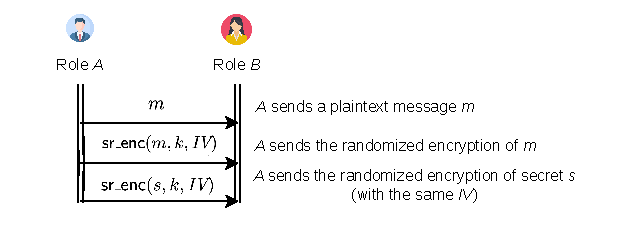
\includegraphics{figs/protocol_iv.pdf}
  \begin{flushleft}\footnotesize
  Protocol in Alice-Bob notation. $\mathsf{sr\_enc}$ denotes symmetric, randomized encryption. 
    \emph{IV} denotes an \emph{initialization vector}, providing a source of randomness for the encryption.
  \end{flushleft}
  \caption{Protocol with IV reuse}
  \label{fig:sr-enc-reuse}
\end{figure}

Symmetric random encryption and decryption is modeled by 
\begin{gather*}
\Sigma = \{ \textsf{sr\_enc} :: \mathit{msg} \times \mathit{msg} \times \mathit{msg} \rightarrow \mathit{msg},\, 
\textsf{sr\_dec} :: \mathit{msg} \times \mathit{msg} \times \mathit{msg} \rightarrow \mathit{msg} \} \text{ and} \\ 
E = \{ \textsf{sr\_dec}(\textsf{sr\_enc}(m, k, \textit{IV}), k) = m \}. 
\end{gather*}
The protocol is computationally insecure, as an initialization vector should never be reused; in this protocol, 
however, $\textit{IV}$ is used in both the second and third message. 
 
More concretely, suppose \textsf{sr\_enc} is defined as follows: 
$\textsf{sr\_enc}(m, k, \textit{IV}) = m \oplus \textsf{keystream}(k, \textit{IV})$, 
where $\oplus$ denotes exclusive or and \textsf{keystream} builds a stream of pseudo-random bits 
from $k$ and $\textit{IV}$ (the details of \textsf{keystream} are not necessary for this discussion). 
In this protocol, the adversary can compute $s$, revealing the secret! 
The derivation is outlined in Figure \ref{fig:d}. 
The initial adversary knowledge is comprised of terms sent along the public channel, 
namely $m$, $\mathsf{sr\_enc}(m, k, \mathit{IV})$, and $\mathsf{sr\_enc}(s, k, \mathit{IV})$.
The derivation outlines how to compute $s$ from these terms, using the definition of 
$\mathsf{sr\_enc}$ and properties of $\oplus$.

\definecolor{grouponeLight}{gray}{0.92}
\definecolor{grouponeDark}{gray}{0.85}

\begin{figure}
    
{\footnotesize

$
\begin{array}{ccc}
  \text{Justification} & \text{Computation}   & \text{Adversary knowledge} \\[.8em]
  \rowcolor{grouponeDark}
  & \green{\mathsf{sr\_enc}(m,k,\mathit{IV})} \oplus \green{m}  & \green{m, \textsf{sr\_enc}(m, k, \mathit{IV})}, \green{\textsf{sr\_enc}(s,k,\mathit{IV})} \\

\rowcolor{grouponeDark}
\text{definition of }\mathsf{sr\_enc} & = (\mathsf{m} \oplus \mathsf{keystream}(k, IV)) \oplus m& \\

\rowcolor{grouponeDark}
\text{commutativity, associativity of }\oplus & = \mathsf{keystream}(k, IV) \oplus (m \oplus m)& \\

\rowcolor{grouponeDark}
\text{cancellation of }\oplus & = \mathsf{keystream}(k, IV) \oplus 0& \\
 
\rowcolor{grouponeDark}
\text{identity of }\oplus & = \purple{\mathsf{keystream}(k, IV)}& \\[.8em]

  \rowcolor{grouponeLight}
  &
  \green{\mathsf{sr\_enc}(s, k, \mathit{IV})} \oplus \green{\mathsf{keystream}(k, \mathit{IV})}    
      & \green{m}, \green{\textsf{sr\_enc}(m, k, \mathit{IV})}, \green{\textsf{sr\_enc}(s,k,\mathit{IV})}, \green{\mathsf{keystream}(k,\mathit{IV})} \\
    \rowcolor{grouponeLight}

  \text{definition of }\mathsf{sr\_enc} &  
  = (s \oplus \mathsf{keystream}(k, \mathit{IV})) \oplus \mathsf{keystream}(k, \mathit{IV}) &  \\ 
  \rowcolor{grouponeLight}
   \text{associativity of }\oplus & 
   = s \oplus (\mathsf{keystream}(k, \mathit{IV}) \oplus \mathsf{keystream}(k, \mathit{IV})) &  \\ 
   \rowcolor{grouponeLight}
   \text{cancellation, identity of }\oplus & 
   = \purple{s}  &  \\ 
\end{array}
$
    
\vspace{.3em}
\green{Green} terms denote terms in the adversary's knowledge at the current step. \newline
\purple{Purple} terms denote terms computed by the adversary in this step. \newline
Black terms denote intermediate terms illustrating the derivation.
\caption{IV reuse attack computing secret $s$}\label{fig:d}
}
\end{figure}

% computes
% sr_enc(s, k, IV) oplus keystream(k, IV) =
% (s oplus keystream(k, IV)) oplus keystream(k, IV) = 
% s oplus (keystream(k, IV) oplus keystream(k, IV))
% = 
% s

However, in the symbolic model, there is no attack, 
as the implementation details of $\textsf{src\_enc}(.,.,.)$ are not specified, and
the attacker \emph{requires} knowledge of $k$ to destruct $\textsf{sr\_enc}(s, k, \textit{IV})$ 
and retrieve $s$. However, $k$ is not derivable by the adversary from the rules in Figure \ref{fig:adv-knowledge}.

\subsection{Symbolic model attacks}\label{sec:sym-attacks} Despite its limitations, 
the symbolic model can still find interesting attacks in practice. 
A famous example is the attack found on the Needham-Schroeder public key authentication protocol \cite{needham_schroeder}, 
which was discovered using cryptographic verification tools 17 years after the protocol was originally published \cite{ns_attack}. 
It uses asymmetric key cryptography, pairing, and projection, modeled by 
\begin{gather*}
\Sigma = \{ \textsf{a\_enc} :: \mathit{msg} \times \mathit{msg} \rightarrow \mathit{msg},\, \textsf{a\_dec} :: \mathit{msg} \times \mathit{msg} \rightarrow \mathit{msg},\, \textsf{pk} :: \mathit{msg} \rightarrow \mathit{msg},\,
\\ \langle ., . \rangle :: \mathit{msg} \times \mathit{msg} \rightarrow \mathit{msg},\,
\pi_1 :: \mathit{msg} \rightarrow \mathit{msg},\, \pi_2 :: \mathit{msg} \rightarrow \mathit{msg} \} \text{ and} \\
E = \{ \textsf{a\_dec}(\textsf{a\_enc}(m, \textsf{pk}(sk)), sk) = m, \pi_1(\langle t_1, t_2 \rangle) = t_1, \pi_2(\langle t_1, t_2 \rangle) = t_2 \}.
\end{gather*}
The protocol is presented in Figure \ref{fig:ns-original}. 

\begin{figure}[t]
  \centering
  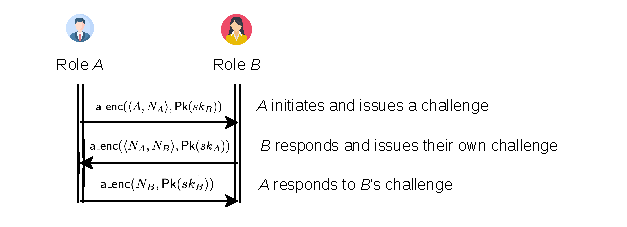
\includegraphics{figs/trace_2.pdf}
  \begin{flushleft}
{\footnotesize
$A$ and $B$ denote protocol roles. $\mathsf{a\_enc}(m, k)$ denotes asymmetric encryption 
with message $m$ and key $k$, and $\mathsf{Pk}(\mathit{sk})$ denotes the public key derived from secret key \emph{sk}.
}
\end{flushleft}
  \caption{The original Needham--Schroeder public-key protocol}
  \label{fig:ns-original}
\end{figure}

The protocol attempts to mutually authenticate $A$ and $B$. Intuitively, from $A$'s perspective, 
$B$ is authenticated because $B$ was able to decrypt the first message with $B$'s secret key and return $N_A$. 
Analogously, from $B$'s perspective, $A$ is authenticated because $A$ was able to decrypt the second message 
with $A$'s secret key and return $N_B$. However, the protocol is symbolically insecure. 
Consider the attack trace with intruder $I$ presented in Figure \ref{fig:ns-lowe-attack}. 
(By inspection, one can verify that all messages sent by $I$ are deducible from the rules in Figure \ref{fig:adv-knowledge}.)

\begin{figure}[t]
  \centering
  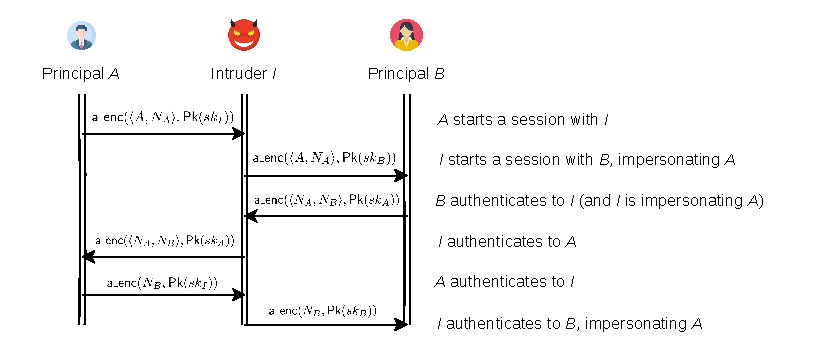
\includegraphics{figs/trace_1.pdf}
    \begin{flushleft}
{\footnotesize
$I$ denotes the intruder. $A$ and $B$ denote principals. $\mathsf{a\_enc}(m, k)$ denotes asymmetric encryption with message $m$ and key $k$, and $\mathsf{Pk}(\mathit{sk})$ denotes the public key derived from secret key \emph{sk}.
}
\end{flushleft}
  \caption{Attack on the original Needham--Schroeder public-key protocol (in Figure \ref{fig:ns-original})}
  \label{fig:ns-lowe-attack}
\end{figure}

Above, $A$ knows that they are communicating with $I$, but $B$ believes that they are communicating with $A$ 
(when $B$ is actually communicating with $I$). 
How was $I$ able to impersonate $A$ to $B$? 
In message $2$, $I$ can simply copy $A$'s challenge because message $1$ was encrypted with $I$'s public key. 
Then $I$ can respond to $B$'s challenge in step $3$ by forwarding it to $A$ in step $4$.

Conceptually, the protocol is insecure because $B$'s challenge is not tied to $B$'s identity---the fix 
is to substitute $\langle N_A, N_B, B \rangle^3$ for $\langle N_A, N_B \rangle$ in step $2$ 
(in Figure \ref{fig:ns-original}).
Here, the superscript $3$ clarifies that the triple constructor is a different constructor 
from the pair constructor (rather than interpreting a triple as nested pairs). 
Then if $I$ forwards in step $4$ (Figure \ref{fig:ns-lowe-attack}), 
it will become clear to $A$ that there is an identity mismatch between $I$ and $B$. 

The Needham-Schroeder protocol is a three-step protocol, and yet it requires care and understanding to avoid symbolic model attacks. Thus, we can argue that for larger and more complicated protocols, symbolic model verification can eliminate relevant classes of attacks, despite its limitations.

\section{Formalizing Protocols in the Symbolic Model}\label{sec:formalizing-protocols}
We aim to mechanize reasoning about cryptographic protocols. To do this, we need to rigorously formalize properties, protocols, and adversarial influence.
Notice that describing protocols as sequences of messages in Alice-Bob notation (as we have done so far) is insufficient for precise reasoning. For example, the encoding leaves the notion of \textit{public knowledge} implicit (e.g., identities and public keys are initially public). Further, it does not describe the \textit{inputs} and \textit{internal steps} of honest participants. Consider a small protocol as in Figure \ref{fig:protocol-small}.

\begin{figure}[h!]
  \centering
  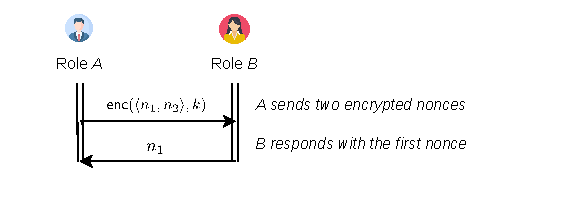
\includegraphics{figs/protocol_small.pdf}
    \begin{flushleft}
      {\footnotesize Alice-Bob notation leaves some paths unspecified---what happens if 
      B cannot retrieve $n_1$?}
\end{flushleft}
  \caption{Ambiguous toy protocol}
  \label{fig:protocol-small}
\end{figure}

 It is left implicit that in the second step, $B$ should decrypt the incoming message, retrieve the first element of the pair $(n_1)$, and send it back to $A$. But what happens if decryption or projection fails? It is not specified.

There are four desirable properties when choosing a formalism to encode protocols and protocol traces in the symbolic model. 
\begin{enumerate}
    \item The formalism must be able to model \emph{message passing} of symbolic terms between parties, taking into account algebraic properties for cryptographic primitives (e.g., equational theory $E$ in Section \ref{sec:sym-threat-model}).
    \item The formalism must be able to encode a \emph{nondeterministic adversary} tampering with communications following a predefined set of capabilities.
    \item The formalism must be able to model the interweaving of multiple distinct sessions, both in parallel and in sequence, allowing the adversary to mix messages of various sessions (say, learning message $m$ from session $1$ and injecting it along the network channel in session $2$).
    \item The formalism would ideally be \textit{executable} in the sense that it should be straightforward to generate protocol traces given a protocol description.
\end{enumerate}
From these requirements, two approaches have historically dominated the formalization of security protocols in the symbolic model: those based on \textit{multiset rewriting}, and those based on \emph{applied} $\pi$\textit{-calculus}. 

\subsection{Multiset rewriting-based approaches}\label{sec:msr-approaches}
The multiset-rewriting approach to cryptographic protocol formalization was pioneered by Durgin and Mitchell in 1999 \cite{msr_foundations}. It is an important formalism for modern automated reasoning techniques in the symbolic model, as it lays the theoretical foundations for Tamarin \cite{tamarin}, a popular symbolic model verification tool.
In this approach, a protocol is a set of multiset rewriting rules, where each rewrite rule can be viewed as a state transition in the protocol. 

\textbf{Formalizing protocols.} We superscript standard set operations with $^\#$ to denote multiset operations (e.g., $\cup^\#$ denotes multiset union and $\in^\#$ for multiset membership). To formalize protocols, we consider another signature $\Sigma_{\textsc{Fact}}$ of \textit{fact symbols}, where \textit{facts} are members of the set $\{ F(t_1, \dots, t_n) \mid F \in \Sigma_{\textsc{Fact}} \;\land\; t_1, \dots, t_n \in T(\Sigma, V \cup \mathcal{N}) \}$. A protocol is represented as a set of rewrite rules $R$, where each rule in $R$ is a triple $(l, a, r)$, where $l, a,$ and $r$ are each finite multisets of facts. Sometimes, we use the alternative notation $l \xrightarrow{a} r$ to denote this triple: $l$ and $r$ respectively represent the left-hand side and right-hand side of the rewrite rule (containing \textit{state facts}), while $a$ represents rule labels (containing \textit{action facts}). 
% More formally, for a protocol $R$, the set of action facts $\mathcal{A}$ 
% is defined as $\{ \mathit{af} \mid \exists a. (\_, a, \_) \in R \land \mathit{af} \in^\# a\}$, 
% and the set of state facts $\mathcal{F}$ 
% is defined as $\{ \mathit{sf} \mid \exists l, r. (l, \_, \_) \in R \land (\_, \_, r) \in R \land (\mathit{sf} \in^\# l \lor \mathit{sf} \in^\# r)\}$. 
For a rewrite rule $l \xrightarrow{a} r$, 
state facts in $l$ are called \emph{premises} and state facts in $r$ are called \emph{conclusions}.
% A wellformedness requirement of protocols is that no fact symbol is used both for some fact in $\mathcal{A}$ and for some fact in $\mathcal{F}$ (so there is no confusion between action facts and state facts). 

\textbf{Formalizing the adversary.} To formalize adversarial behavior, we assume the existence of four special fact symbols \textsf{In}, \textsf{Out}, \textsf{Fr}, and \textsf{K}. \textsf{In} and \textsf{Out} are included in the protocol's rules to model taking input and sending output to the insecure network channel. \textsf{Fr} represents fresh variables (where freshness is later enforced in the operational semantics), and \textsf{K} represents adversary knowledge and should not be present in protocol rules.
Adversarial behavior can be captured by a fixed set of rewrite rules \textsf{Adv} that roughly mirror the rules in Figure \ref{fig:adv-knowledge}. \textsf{Adv} is defined in Figure \ref{fig:adv-rules}: the first three rules on the left correspond to \textsc{Net}, \textsc{Fr}, and \textsc{Pub}, respectively; the last rule on the left corresponds to the adversary's capability to inject messages on the network; and the rules on the right correspond to \textsc{Fun}.

In the last rule on the left in Figure \ref{fig:adv-rules}, the bang ($!$) is shorthand to denote that the fact should be repeated on the right-hand side of the rule. Facts with bangs are called \textit{persistent facts}, as they represent persistent state. For clarity, a fact should never be persistent in one rule and \textit{linear} (i.e., not persistent) in another rule.

\begin{figure}[t]
  \centering
  \[
  \textsf{Adv} \;=\;
  \left\{
  \begin{array}{rcl}
    \{ \mathsf{Out}(x) \}
      & \xrightarrow{\{\}} &
    \{ \mathsf{K}(x) \} \\[2pt]

    \{ \mathsf{Fr}(\blue{x}) \}
      & \xrightarrow{\{\}} &
    \{ \mathsf{K}(\blue{x}) \} \\[2pt]

    \{ \}
      & \xrightarrow{\{\}} &
    \{ \mathsf{K}(x^\textsc{pub}) \} \\[2pt]

    \{ !\mathsf{K}(x) \}
      & \xrightarrow{\{\mathsf{K}(x)\}} &
    \{ \mathsf{In}(x) \} 
  \end{array}
  \right\}
  \;\cup\;
  \left\{
  \begin{array}{l}
    \{ \mathsf{K}(t_1), \dots, \mathsf{K}(t_n) \}
      \xrightarrow{\{\}}
    \{ \mathsf{K}(f(t_1, \dots, t_n)) \} \\[2pt]
    \qquad\text{for all } (f,n) \in \Sigma
  \end{array}
  \right\}
  \]
  \begin{flushleft}
{\footnotesize
Each triple $l \xrightarrow{a} r$ denotes a multiset rewriting rule from $l$ to $r$ with labels $a$. \textsf{Out} (resp., \textsf{In}) denotes output (resp., input) along the network channel, \textsf{Fr} denotes fresh terms, and \textsf{K} denotes intruder knowledge.
}
  \end{flushleft}
  
  \caption{Adversary rules for multiset rewriting formalization}
  \label{fig:adv-rules}
\end{figure}

\textbf{Protocol traces.} A protocol trace is a sequence of states, where each successive pair of states follows from one of the rules in $R \cup \mathsf{Adv} \cup \{ \mathsf{Fresh} \}$, where $\mathsf{Fresh}$ denotes the built-in rule for fresh variables $\{\} \xrightarrow{\{\}} \{ \mathsf{Fr}(x) \}$. 
More formally, we use $\sigma$ to denote a substitution from variables to terms;
we abuse notation and also use postfix notation $m\sigma$ to denote the application of (the homomorphic extension of) $\sigma$ to all arguments of all facts in multiset $m$.
We further abuse notation
and write $\sigma_1 \circ \sigma_2$ to denote the composition of substitutions, where we apply the homomorphic extension of $\sigma_2$ to the output $\sigma_1$ (which itself may also be interpreted as a homomorphic extension depending on context).
Let $\mathsf{ginsts}(l \xrightarrow{a} r)$ denote the ground instances of a rewrite rule $l \xrightarrow{a} r$, 
i.e., $$\mathsf{ginsts}(l \xrightarrow{a} r) = \{ l_g \xrightarrow{a_g} r_g \mid \exists \sigma.\; l \sigma = l_g \land  a \sigma = a_g \land r \sigma = r_g \land \sigma \text{ only maps to ground terms} \}.$$ 
Further, we use $\mathsf{ginsts}_E(l \xrightarrow{a} r)$ to denote the ground instances of $l \xrightarrow{a} r$ modulo equational theory $E$, 
i.e.,  $$\mathsf{ginsts}_E(l \xrightarrow{a} r) = \{ l' \xrightarrow{a'} r' \mid \exists l_g \xrightarrow{a_g} r_g \in \mathsf{ginsts}(l \xrightarrow{a} r) \land l' =_E l_g \land a' =_E a_g \land r' =_E r_g \}.$$ 
Finally, we lift $\mathsf{ginsts}_E(.)$ from single rewrite rules to sets of rewrite rules as expected. 
From this, we can define a small-step labeled transition relation for a set of rewrite rules $R$, 
denoted $\xrightarrow{a}_R$, with the following inference rule. 
Here, assume $S$ denotes the current state (which is a multiset of facts) and $\mathcal{S}$ denotes the set of all states, 
and hence $\xrightarrow{a}_R \;\subseteq \mathcal{P}(\mathcal{S}) \times \mathcal{P}(\mathcal{S})$. 
  \begin{mathpar}
    \inferrule*
      { l \xrightarrow{a} r \in \mathsf{ginsts}_E(R) \quad l \subset^\# S }
      { S \xrightarrow{a}_R (S  \setminus ^\# l) \cup^\# r }
  \end{mathpar}
Intuitively, the state $S$ evolves at each step through the application of some rewrite rule in $R$ that consumes state facts on the left-hand side of the rule and produces state facts on the right-hand side of the rule.
Finally, a \textit{trace} of a protocol $R$ is a sequence of states $S_0, \dots, S_n$ such that $S_0 = \emptyset$ and $S_i \xrightarrow{a}_R S_{i+1}$ for all $i$ (for some $l \xrightarrow{a} r \in \mathsf{ginsts}_E(R)$), with the additional well-formedness requirement that the rule $\{\} \xrightarrow{\{\}} \{ \mathsf{Fr}(x) \}$ is used at most once for a given instantiation of $x$.

\textbf{Example protocol formalization.} We will formalize the (insecure) Needham Schroeder protocol from Figure \ref{fig:ns-original}, as well as the attack trace. Consider 
\begin{gather*} 
\Sigma = \{ \mathsf{a\_enc} :: \mathit{msg} \times \mathit{msg} \rightarrow \mathit{msg},\, \mathsf{a\_dec} :: \mathit{msg} \times \mathit{msg} \rightarrow \mathit{msg},\, \mathsf{pk} :: \mathit{msg} \rightarrow \mathit{msg},\, \\ \langle ., . \rangle :: \mathit{msg} \times \mathit{msg} \rightarrow \mathit{msg},\, 
\pi_1 :: \mathit{msg} \rightarrow \mathit{msg},\, \pi_2 :: \mathit{msg} \rightarrow \mathit{msg}  \}, \\
E = \{ \mathsf{a\_dec}(\mathsf{a\_enc}(m, \mathsf{pk}(k)), k) = m, \pi_1(\langle t_1, t_2 \rangle) = t_1, \pi_2(\langle t_1, t_2 \rangle) = t_2 \}, \text{ and } \\ \Sigma_{\textsc{Fact}} = \{ \mathsf{In} :: \mathit{msg},\, \mathsf{Out} :: \mathit{msg},\, \mathsf{Fr} :: \mathit{fr},\, \mathsf{K} :: \mathit{msg},\, \mathsf{Pk} :: \mathit{msg} \times \mathit{msg},\, \mathsf{Ltk} :: \mathit{msg} \times \mathit{msg},\, \\
\mathsf{StA1} :: \mathit{msg} \times \mathit{msg} \times \mathit{msg},\, \mathsf{StB1} :: \mathit{msg} \times \mathit{msg} \times \mathit{msg} \times \mathit{msg},\, \mathsf{StA2} :: \mathit{msg} \times \mathit{msg} \times \mathit{msg} \times \mathit{msg} \}.
\end{gather*}
The protocol is encoded as a set of rewrite rules $R = \{ \mathsf{Register}, A_1, B_1, A_2, B_2 \}$, 
where the rewrite rules are defined as in Figure 8.
\begin{figure}[t]
  \centering
\begin{align*}
\mathsf{Register}
&\triangleq \{ \mathsf{Fr}(\blue{sk}) \}
   \xrightarrow{\{\}} \\ 
&\hspace{14pt}
   \{ \mathsf{Ltk}(\red{A}, \blue{sk}),
      \mathsf{Pk}(\red{A}, \mathsf{pk}(\blue{sk})),
      \mathsf{Out}(\langle \red{A}, \mathsf{pk}(\blue{sk}) \rangle) \},
\\[0.5em]
\mathsf{Reveal}
  &\triangleq \{ \mathsf{!Ltk}(\red{A}, \blue{sk}) \}
   \xrightarrow{\{\}} \\ 
&\hspace{14pt}
   \{ \mathsf{Out}(\blue{sk}) \},
\\[0.5em]
A_1
&\triangleq \{ \mathsf{Fr}(\blue{n_A}),
      !\mathsf{Pk}(\red{A}, \red{pk_A}),
      !\mathsf{Pk}(\red{B}, \red{pk_B}) \} \xrightarrow{\{\}}
\\
& 
   \hspace{14pt} \{ \mathsf{StA1}(\red{A}, \red{B}, \blue{n_A}), \mathsf{Out}(\mathsf{a\_enc}(\langle \red{A}, \blue{n_A} \rangle, \red{pk_B})) \},
\\[0.5em]
B_1
&\triangleq \{ \mathsf{In}(c),
      !\mathsf{Ltk}(\red{B}, \blue{sk_B}),
      !\mathsf{Pk}(\red{A}, \red{pk_A}),
      \mathsf{Fr}(\blue{n_B}) \} \xrightarrow{\{\}}
\\
& 
   \hspace{14pt}\{ \mathsf{StB1}\!\left(
        \red{B},
        \pi_1(\mathsf{a\_dec}(c, \blue{sk_B})),
        \pi_2(\mathsf{a\_dec}(c, \blue{sk_B})),
        \blue{n_B}
      \right),
\\
& 
     \hspace{28pt}\mathsf{Out}\!\left(
        \mathsf{a\_enc}(
          \langle \pi_2(\mathsf{a\_dec}(c, \blue{sk_B})), \blue{n_B} \rangle,
          \red{pk_A}
        )
      \right)
   \},
\\[0.5em]
A_2 
&\triangleq \{ \mathsf{In}(\textsf{a\_enc}(\langle \blue{n_A}, \blue{n_B} \rangle, pk(\blue{sk_A}))),
      !\mathsf{Ltk}(\red{A}, \blue{sk_A}),
      !\mathsf{Pk}(\red{B}, \red{pk_B}),
      \mathsf{StA1}(\red{A}, \red{B}, \blue{n_A}) \} \xrightarrow{\{\mathsf{Sent}(\red{A}, \red{B}, \blue{n_A}, \blue{n_B})\}}
\\
& 
   \hspace{14pt}\{ \mathsf{StA2}\!\left(
        \red{A},
        \red{B},
        \blue{n_A},
        \blue{n_B}
      \right),
\\
& 
      \hspace{28pt}\mathsf{Out}\!\left(
        \mathsf{a\_enc}(
          \blue{n_B},
          \red{pk_B}
        )
      \right)
   \}, \text{ and}
\\[0.5em]
B_2
&\triangleq \{ \mathsf{In}(\mathsf{a\_enc}(\blue{n_B}, \mathsf{pk}(\blue{sk_B}))),
      !\mathsf{Ltk}(\red{B}, \blue{sk_B}),
      \mathsf{StB1}(\red{B}, \red{A}, \blue{n_A}, \blue{n_B}) \} \xrightarrow{\{\mathsf{Accept}(\red{B}, \red{A}, \blue{n_A}, \blue{n_B})\}}
\\
& 
   \hspace{14pt}\{  \}.
\end{align*}
\label{fig:ns-rules-test}
\begin{flushleft}
{\footnotesize 
Each triple $l \xrightarrow{a} r$ denotes a multiset rewriting rule from $l$ to $r$ with labels $a$, and facts with ``!" denote persistent facts. For example,  \textsf{Register} is the name of a rewrite rule that consumes $\mathsf{Fr}(\blue{\mathit{sk}})$ from the state (i.e., a fresh secret key) and introduces to the state a longterm key (stored in $\mathsf{Ltk(.,)}$), a public key (stored in $\mathsf{Pk}(.,.)$), and network channel output (stored in $\mathsf{Out}(.)$).
}
\end{flushleft}
\caption{Rewrite rules formalizing Figure \ref{fig:ns-original}}
\end{figure}

The first rule, \textsf{Register}, represents the registration of an asymmetric key pair to identity 
$A$. Note that $A$, 
along with the other identifiers in the rule descriptions, 
are \textit{variables} and can be instantiated with different values 
in different rule instances. 
Hence, the protocol description can capture an unbounded number of sessions and principals. 
The \textsf{Ltk} (short for ``long-term key") stores $A$'s (fresh) 
secret key $sk$, while $\textsf{Pk}$ stores the public key derived from $sk$. 
Finally, the identity/public key mapping are broadcast along the network channel, 
as they are public information that should be known by the adversary for realistic modeling.

The second rule, \textsf{Reveal}, leaks a secret key on the network channel. This models \emph{key compromise}, 
a situation where one or more of the secret keys leaked to the adversary. 
A rule for revealing keys tests the \emph{compromise resilience} of a protocol---one can test the security 
of a protocol with limitations imposed on the \textsf{Reveal} rule (unrestricted use trivially compromises security).
In the attack on the Needham-Schroeder protocol, \textsf{Reveal} is needed to give intruder $I$ knowledge of their own secret
key; however, the attack does not rely on revealing the secret key of honest role $A$ or $B$.

Rules $A_1$, $B_1$, $A_2$, and $B_2$ closely mirror the rules in Figure \ref{fig:ns-original}; 
however, they explicitly reference state to retrieve the corresponding keys. 
Terms can be destructed either with destructor symbols (as in $B_1$) or by pattern 
matching on inputs (as in $A_2$ and $B_2$).
Additionally, state fact symbols \textsf{StA1}, \textsf{StB1}, and \textsf{StA2} 
are used to ensure that protocol traces follow \textit{ordering constraints} 
(i.e., that protocol rule $i$ is executed before protocol rule $i+1$ in a given session), 
as well as to store information about the current session.
Notice that in $A_2$ and $B_2$, pattern matching is used to implicitly impose 
equality constraints (for example, in $A_2$, the $n_A$ returned by $B$ on the network channel matches the $n_A$ 
stored in \textsf{StA1}).
Action facts \textsf{Accept} and \textsf{Sent} can later be used to help state 
an injective or non-injective agreement property.

Rule $B_2$ is used to explicitly denote cases where $B$ believes that $B$ has 
completed a protocol session with $A$. 

\textbf{Example protocol trace formalization.}
We can now formalize the attack trace in Figure \ref{fig:ns-lowe-attack} as a trace of $R \cup \mathsf{Adv} \cup \{ \mathsf{Fresh} \}$ (see Figure \ref{fig:ns-lowe-attack-ms-prefix}). 
The full trace is far too verbose 
to be useful; 
we outline the first few steps representing key generation. 
At each step, we outline the rule used and the updates to state (a multiset of ground facts).

\begin{figure}[h]
\centering
\small
\begin{tabular}{p{8cm}p{8cm}}

\textbf{Rule application} & \textbf{State} \\
\rowcolor{grouponeDark}
NA &
$S_0 = \emptyset$
\\[0.8em]

\rowcolor{grouponeLight}
$\{\} \xrightarrow{\{\}} \{\mathsf{Fr}(\blue{sk_A})\}$ &
$\{\mathsf{Fr}(\blue{sk_A})\}$
\\[0.8em]

\rowcolor{grouponeDark}
$\{\mathsf{Fr}(\blue{sk_A})\} \xrightarrow{\{\}}$ \newline
$\{\mathsf{Ltk}(\red{A},\blue{sk_A}),\mathsf{Pk}(\red{A},\mathsf{pk}(\blue{sk_A})),
\mathsf{Out}(\langle \red{A},\mathsf{pk}(\blue{sk_A})\rangle)\}$ &
$\{\mathsf{Ltk}(\red{A},\blue{sk_A}),
\mathsf{Pk}(\red{A},\mathsf{pk}(\red{sk_A})),
\mathsf{Out}(\langle \red{A},\mathsf{pk}(\blue{sk_A})\rangle)\}$
\\[1.6em]

\rowcolor{grouponeLight}
$\{\} \xrightarrow{\{\}} \{\mathsf{Fr}(\blue{sk_I})\}$ &
$\{\mathsf{Ltk}(\red{A},\blue{sk_A}),
\mathsf{Pk}(\red{A},\mathsf{pk}(\blue{sk_A})),
\mathsf{Out}(\langle \red{A},\mathsf{pk}(\blue{sk_A})\rangle),
\mathsf{Fr}(\blue{sk_I})\}$
\\[0.8em]

\rowcolor{grouponeDark}
$\{\mathsf{Fr}(\blue{sk_I})\} \xrightarrow{\{\}}$\newline
$\{\mathsf{Ltk}(\red{I},\blue{sk_I}),\mathsf{Pk}(\red{I},\mathsf{pk}(\blue{sk_I})),
\mathsf{Out}(\langle \red{I},\mathsf{pk}(\blue{sk_I})\rangle)\}$ &
$\{\mathsf{Ltk}(\red{A},\blue{sk_A}),
\mathsf{Pk}(\red{A},\mathsf{pk}(\blue{sk_A})),
\mathsf{Out}(\langle \red{A},\mathsf{pk}(\blue{sk_A})\rangle),$ \newline
$\mathsf{Ltk}(\red{I},\blue{sk_I}),
\mathsf{Pk}(\red{I},\mathsf{pk}(\blue{sk_I})),
\mathsf{Out}(\langle \red{I},\mathsf{pk}(\blue{sk_I})\rangle)\}$\\[1.6em]
\rowcolor{grouponeLight}
... & ...
\end{tabular}
\begin{flushleft}
\vspace{.3em}
{\footnotesize
   The left column outlines a sequence of ground instantiations of multiset rewriting rules denoting a trace prefix, and the right column outlines the corresponding updates to the state. Each rewrite rule consumes facts from the state (on the left-hand of the rule) and introduces new facts to the state (on the right-hand side of the rule).
    }
\end{flushleft}
  \caption{ Needham--Schroeder public-key protocol attack as multiset rewriting protocol trace prefix}
  \label{fig:ns-lowe-attack-ms-prefix}
\end{figure}

\textbf{Security property formalization.} In this setting, given a protocol $R$, weak secrecy of a term $t$ is phrased in terms of the existence of some protocol trace with some step $S_i \xrightarrow{\mathsf{K}(t)} S_{i+1}$ (where $t$ is in the adversary's knowledge base, captured by action fact $\mathsf{K}(t)$). That is, a protocol satisfies weak secrecy of $t$ if there is no trace with such a step.

More concretely, we consider security properties $\varphi$ in a variant of first-order logic with equality that replaces predicates $p(t_1, \dots, t_n)$ with \textit{actions} of the form $f(t_1, \dots, t_n)@i$ (where $f(t_1, \dots, t_n)$ is some action fact, and $i$ is a temporal variable).
In this logic, we define a satisfaction relation $\mathit{tr}, \theta \models_E \varphi$ which means that trace \emph{tr} with valuation $\theta$ satisfies formula $\varphi$, modulo equational theory $E$. More details of this property specification logic will be described in Section \ref{sec:mechanized-reasoning}.

%All x #i. Secret(x) @i ==> not (Ex #j. K(x)@j)
As an intuitive example, one can specify a secrecy property as the first-order logic formula $\forall x. \; \forall i. \; \mathsf{Secret}(x) @i \Rightarrow \neg (\exists j. \mathsf{K}(x)@j)$. 
Intuitively, if $x$ is marked as secret by some action fact in the protocol description (at any time $i$), 
then $x$ does not appear in the adversary's knowledge base (at any time $j$).

\subsection{$\pi$-calculus-based approaches}\label{sec:apc-approaches}
Symbolic model protocol analysis approaches based on $\pi$-calculus were pioneered by Abadi and Fournet in \cite{apc}, and lay the theoretical foundations for the popular automated reasoning tool ProVerif \cite{proverif}. Additionally, many theoretical results in symbolic model verification (discussed in Section \ref{sec:tractable-reasoning}) are expressed in terms of the $\pi$-calculus. Intuitively, the $\pi$-calculus is a minimal language that captures the concurrent execution of a collection of processes with message passing of atomic names, also supporting the dynamic creation of new communication channels.

When reasoning about cryptographic protocols, we use an extension of the $\pi$-calculus, called the \textit{applied $\pi$-calculus}, where processes exchange symbolic terms in addition to atomic channel names. These terms represent cryptographic messages, and we can use the same set of terms $\mathcal{T}(\Sigma, D)$ as in the multiset rewriting formalization, except that $D$ also contains channel names.

\textbf{$\pi$-calculus preliminaries.} An evaluation context $C$ is a process with a hole (denoted $\square$) in it, and $C[P]$ denotes filling the hole in $C$ with process $P$. For example, with context $C \triangleq \textsf{if } M = N \textsf{ then } \square \textsf{ else } P$, then $C[0]$ denotes $\textsf{if } M = N \textsf{ then } 0 \textsf{ else } P$.

\textbf{Syntax.} Below is the grammar for \textit{plain processes}, where $c$ ranges over channel names and variables, $n$ over names, $x$ over variables, and $M$ and $N$ over terms.

$
\begin{array}{ll}
    P ::=  & \text{plain processes} \\ 
    \quad 0  & \quad\text{null process} \\ 
    \quad P_1 \mid P_2 & \quad\text{parallel composition} \\ 
    \quad !P & \quad\text{replication} \\ 
    \quad \textbf{\textsf{new }} n.\; P & \quad\text{name restriction} \\ 
    \quad \textsf{if } M=N \textsf{ then } P_1 \textsf{ else } P_2 & \quad\text{conditional} \\ 
    \quad c(x).P & \quad\text{message input on channel }c \\ 
    \quad \bar{c}\langle N \rangle.P & \quad\text{message output on channel }c
\end{array}
$

It is close to standard $\pi$-calculus, except for sending terms (rather than just atomic names) as output, 
as well as conditionals with equality tests on terms. 
Intuitively, the null process does nothing; 
parallel composition refers to two processes executing (asynchronously) in parallel;
the replication of $P$ spawns arbitrarily many copies of $P$;
the name restriction $\textbf{\textsf{new }} n.\;P$ creates a fresh name and binds it to $n$ before proceeding with $P$; 
the conditional performs an equality check to then proceed with the corresponding branch; 
the message input $c(x).P$ takes a message sent along $c$ and binds it to $x$ before proceeding with $P$; 
and the message output $\bar{c}\langle N \rangle.P$ sends message $N$ on channel $c$ before proceeding with $P$.

Additionally, we introduce substitutions of the form $\{ x \mapsto M \}$ directly into the core language, where $x$ is a variable and $M$ is a term. To distinguish object-level substitutions from meta-level substitutions, we call object-level substitutions \emph{active substitutions}. The set of a process's active substitutions can be viewed as the \textit{adversary knowledge}. Intuitively, the adversary process can sample fresh terms and use terms in scope (i.e., in its knowledge), but terms outside of the set of active substitutions (like unleaked secret keys) are not guessable.

$
\begin{array}{ll}
    Q ::=  & \text{extended processes} \\ 
    \quad P  & \quad\text{plain process} \\ 
    \quad Q_1 \mid Q_2 & \quad\text{parallel composition} \\ 
    \quad \textbf{\textsf{new }} n.\; Q & \quad\text{name restriction} \\ 
    \quad \textbf{\textsf{new }} v.\; Q & \quad\text{variable restriction} \\ 
    \quad \{ x \mapsto M\} & \quad\text{active substitution} 
\end{array}
$

\textbf{Structural equivalence.} The first step to defining the operational semantics of the applied $\pi$-calculus is to define \textit{structural equivalence} $\equiv$, a binary relation that intuitively captures the equivalence of two processes without taking forward steps of computation (i.e., the structural equivalence rules may be applied in both directions). 

$\equiv$ is defined as the smallest relation closed under $\alpha$-renaming on bound names and variables, and by application of evaluation contexts, containing the following pairs. Below, $\mathit{fn}(P)$ denotes the free names of $P$.

{\footnotesize
$
\begin{array}{crcll}
(1) & A & \equiv & A \mid 0 & \text{null process}\\
(2) & A \mid (B \mid C) & \equiv & (A \mid B) \mid C & \text{associativity of parallel composition}\\ 
(3) & A \mid B & \equiv & B \mid A  & \text{commutativity of parallel composition}\\ 
(4) & !P & \equiv & P \mid \;!P & \text{replication}\\ 
(5) & \textbf{\textsf{new }}n. \; 0 & \equiv & 0 & \text{restriction over the null process}\\
(6) & \textbf{\textsf{new }}n_1. \; \textbf{\textsf{new }}n_2. \;Q & \equiv & \textbf{\textsf{new }}n_2. \; \textbf{\textsf{new }}n_1. \;Q & \text{commutativity of restrictions}\\
(7) & Q_1 \mid \textbf{\textsf{new }}n.\; Q_2 & \equiv & \textbf{\textsf{new }}n.\;(Q_1 \mid Q_2) \text{ (when } n \not\in (\mathit{fv}(Q_1)\cup \mathit{fn}(Q_1)) \text{)} & \text{scope extension of restriction}\\ 
(8) & \textbf{\textsf{new }}x.\;\{x \mapsto M\} & \equiv & 0 & \text{restriction of active substitution}\\ 
(9) & \{x\mapsto M\} \mid A & \equiv & \{x\mapsto M\} \mid A\{x\mapsto M\} & \text{application of active substitution}\\ 
(10) & \{x\mapsto M\} & \equiv & \{x\mapsto N\} \text{ (when } M =_E N \text{)}& \text{equational reasoning on substitutions}
\end{array}
$}

Cases (1) through (7) are standard in $\pi$-calculus. Case (8) intuitively captures the idea that an active substitution for a fresh variable $x$, with no other processes in scope to use $x$, cannot directly perform computation. Case (9) denotes the application of an active substitution. Case (10) captures the interchangeability of $M$ and $N$ when $M =_E N$ (note that we can use the same notion of $=_E$ from Section \ref{sec:msr-approaches}).

\textbf{Operational semantics.} We define a small-step relation $\rightarrow$, which is the smallest relation closed under structural equivalence and evaluation contexts such that the following hold. 

$
\begin{array}{crcll}
(1)  & \bar{c}\langle x \rangle.\; Q_1 \mid c(x).\; Q_2 & \rightarrow & Q_1 \mid Q_2 & \text{message passing}\\
(2)  & \textsf{if } M = M \textsf{ then } Q_1 \textsf{ else } Q_2 & \rightarrow & Q_1  & \text{then branch}\\
(3)  & \textsf{if } M = N \textsf{ then } Q_1 \textsf{ else } Q_2 & \rightarrow & Q_2 \text{ (when } M \neq_E N \text{)}  & \text{else branch}\\
\end{array}
$

Above, rule (1) represents sharing a message across a shared channel $c$. 
It might seem strange to require a variable (rather than any term) to be sent along $c$. 
However, this restriction is without loss of generality because a process can send term $M$ 
by introducing a fresh variable $x$ and active substitution $\{x\mapsto M\}$ using the structural equivalence rules above. 

\textbf{Example protocol.} 
We encode the original Needham-Schroeder protocol from Figure \ref{fig:ns-original} 
in the applied $\pi$-calculus. 
For clarity, we introduce a few aspects of syntactic sugar. 
First, we  introduce \textit{let expressions} of the form 
$\textsf{let }x = e_1 \textsf{ in } e_2$. 
Second, we introduce \textit{abstractions} of the form $\mathsf{Name}(x_1, \dots, x_n) \triangleq P[x_1, \dots, x_n]$, 
which are functions from terms to processes and can be called with the usual syntax 
$\mathsf{Name}(t_1, \dots, t_n)$. 
A let expression $\textsf{let } x = e_1 \textsf{ in } e_2$
is syntactic sugar that is eliminated by syntactically replacing every free occurrence of x
in $e_2$ with $e_1$ (and analogously for abstractions).
Additionally, we can pattern match on input terms (e.g., $c(\langle A, n_A \rangle)$), 
which we implement as sugar for taking a fresh variable as input and using let expressions to define 
variables introduced by pattern matching before proceeding
(here, replacing $c(\langle A, n_A \rangle).P$ with 
${c}(x).\textsf{let }A = \pi_1(x) \textsf{ in } \textsf{let }n_A = \pi_2(x) \textsf{ in } P$).

\[
\begin{aligned}
\mathsf{Initiator}(\red{A},\blue{sk_A})
&\;\triangleq\;
c(\langle \red{B}, \red{pk_B}\rangle).\;
\textbf{\textsf{new }} \blue{n_A}.\;
\bar{c}\langle \mathsf{a\_enc}(\langle \red{A}, \blue{n_A} \rangle, \red{pk_B}) \rangle .
\\
&\hspace{4em}
c(x).\;
\textsf{let } m_2 = \mathsf{a\_dec}(x, \blue{sk_A}) \textsf{ in }
\\
&\hspace{4em}
\textsf{if } \pi_1(m_2) = \blue{n_A} \textsf{ then }
\big(
  \textsf{let } \blue{n_B} = \pi_2(m_2) \textsf{ in }
  \bar{c}\langle \mathsf{a\_enc}(\blue{n_B}, \red{pk_B}) \rangle . 0
\big)
\\
&\hspace{4em}
\text{else } 0
\\[1.0em]
\mathsf{Responder}(\red{B},\blue{sk_B})
&\;\triangleq\;
c(y).\;
\textsf{let } m_1 = \mathsf{a\_dec}(y, \blue{sk_B}) \textsf{ in }
\\
&\hspace{4em}
\textsf{let } \red{A'} = \pi_1(m_1) \textsf{ in }
\textsf{let } \blue{n_A} = \pi_2(m_1) \textsf{ in }
\textbf{\textsf{new }} \blue{n_B}.\;
c(\langle \red{A''}, \red{pk_A}\rangle).\;
\\
&\hspace{4em}
\textsf{if } \red{A''} = \red{A'} \textsf{ then }
\\
&\hspace{6em}
\bar{c}\langle \mathsf{a\_enc}(\langle \blue{n_A}, \blue{n_B} \rangle, \red{pk_A}) \rangle .\; 
  c(z).\;
  \textsf{let } m_3 = \mathsf{a\_dec}(z, \blue{sk_B}) \textsf{ in }
  \\
  &\hspace{6em}
  \textsf{if } m_3 = \blue{n_B} \textsf{ then } \bar c \langle \mathsf{ok} \rangle.0 \textsf{ else } 0
\\&\hspace{4em}
\textsf{ else } 0
\\[1.0em]
\mathsf{Principal}
&\;\triangleq\;
\textbf{\textsf{new }}\red{A}.\;\textbf{\textsf{new }}\blue{sk_A}.\;
\bar{c}\langle \langle \red{A}, \mathsf{pk}(\blue{sk_A}) \rangle \rangle .
\big(\; !\mathsf{Initiator}(\red{A},\blue{sk_A})\ \mid\ !\mathsf{Responder}(\red{A},\blue{sk_A})\;\big)
\\[1.0em]
\mathsf{System}
&\;\triangleq\;
!\mathsf{Principal}
\end{aligned}
\]

Above, the $\mathsf{Principal}$ process loops on both roles, $\mathsf{Initiator}$ and $\mathsf{Responder}$, 
with a fixed identity $A$ (i.e., principal $A$ runs unbounded sessions of both roles). 
Because the top-level $\mathsf{System}$ replicates $\mathsf{Principal}$, we also get unbounded principals. 
$\mathsf{Initiator}$ retrieves an identity $B$ and public key $pk_B$ along $c$ (sent by $\textsf{Principal})$ 
and starts a new session with fresh nonce $n_A$, sending the first message along the network channel with 
$\bar c \langle \mathsf{a\_enc}(\langle A, n_A \rangle,pk_B)\rangle$. 
Then, it takes the response (from $B$) as input from the network with $c(x)$, 
decrypts the incoming message, and checks if the response correctly returns $n_A$. 
If so, it retrieves $B$'s challenge nonce $n_B$ and returns its encryption along $\bar c$. 
If decryption fails or if $n_A$ is not returned, the guard $\pi_1(m_2) = n_A$ will fail (as $\pi_1(m_2) \neq_E n_A$) 
and the initiator will stall at the empty process rather than sending the last message. 
One can trace the $\mathsf{Responder}$'s logic playing role $B$ in an analogous fashion. 
Notice that we are emitting a special term $\textsf{ok}$ to denote that the \textsf{Responder} 
successfully finished a protocol session to make it observationally distinguishable from the case 
where the session was unsuccessful. 
This idea will be expanded in Section \ref{sec:mechanized-reasoning} with the discussion of \emph{events}.

The above encoding has an attack not present in the informal protocol description. Since the identity to public key mapping $\langle A, \mathsf{pk}(sk_A)\rangle$ is sent along the public network channel (by \textsf{Principal}), the attacker can simply replace $A$'s public key with his own, i.e. $\langle A, \mathsf{pk}(sk_I)\rangle$. Modern cryptosystems prevent this attack with a separate mechanism involving \textit{certificates} and \textit{certificate validation}, but this is out of scope for this document, and ID to public key mappings are usually assumed secure for the purposes of protocol analysis.
To disallow this attack, one must extend the applied $\pi$-calculus syntax and semantics to support additional features---either a private channel to prevent adversarial tampering, or a global constant providing an ID to public key mapping that can be directly referenced by protocol participants.

\textbf{Security properties.}
Security properties in the applied $\pi$-calculus setting are traditionally phrased in terms of 
\textit{observational equivalences} between processes, 
where observational equivalence is defined in terms of \textit{barbs}. 
Intuitively, a channel $c$ is a \textit{barb} for process $P$ if $P$ is capable of sending some message along $c$. 
More formally, channel $c$ is a \textit{barb} for process $P$ if, for some term $M$, 
$P \rightarrow^* C[\bar{c}\langle M \rangle]$  for some context $C$ such that $c$ is not bound in $C$. 
We denote ``$c$ is a barb for $P$" as $P \Downarrow c$. Then, we can define \textit{observational equivalence} 
$(\approx)$ as the largest symmetric relation between closed extended processes such that $P \approx Q$ implies
\begin{enumerate}
    \item[$(i)$] if $P \Downarrow c$ for some $c$, then $Q \Downarrow c$;
    \item[$(ii)$] if $P \rightarrow^* P'$, then there exists some $Q'$ such that $Q \rightarrow^* Q'$ and $P' \approx Q'$; and
    \item[$(iii)$] $C[P] \approx C[Q]$ for all contexts $C$.
\end{enumerate}

Now consider a process $P[s]$ that is supposed to keep free variable $s$ secret 
(e.g., $s$ is encrypted and sent along a channel). 
We say that $P$ satisfies the (strong) secrecy of $s$ if for all terms $t$ and  $t'$, $P{s \mapsto t} \approx P{s \mapsto t'}$.

While we did not explicitly encode attacker rules as in Figure \ref{fig:adv-rules}, 
the attacker is played by the arbitrary context $C$ in point $(iii)$ above. 
Consider the strong secrecy of $s$ in this small process: 
$P(s) \triangleq \textsf{if }s = \textsf{N}\textsf{ then } \bar c \langle \mathsf{ok} \rangle 
\textsf{ else } \bar c \langle \mathsf{ko} \rangle $ (assume \textsf{ok},  \textsf{ko}, and \textsf{N} are concrete constants). 
Here, $P(s)$ branches on $s$, but it never reveals it on the channel. Here, context $C$ can distinguish $c$ 
from any other value for $s$, where 
$C[\square] \triangleq (\square \mid c(M). \textsf{if }M=\textsf{ok} \textsf{ then } \bar d(\textsf{ok}) \textsf{ else } 0.)$ 
In general, the adversary can perform always perform \emph{tests} in the guard of \textsf{if} expressions 
and emit a barb in one case and not in the other. Here, $C[P(\mathsf{N})]$ gives a barb on $d$, 
while $C[P(x)]$ (with $x \neq \mathsf{N}$) does not give a barb on $d$, hence breaking the observational equivalence. 
Note that an evaluation context $C$ intuitively has the same capabilities as a symbolic adversary shown 
in Figure \ref{fig:adv-knowledge}---the active substitutions give the context access to public terms; 
the adversary can apply function symbols to terms in scope; 
the adversary can sample fresh terms with \textbf{\textsf{new}}; 
the adversary can use the guard to \textsf{if} expressions to reason equationally;  
and the adversary \emph{cannot} directly reference terms that are out of scope (e.g., secrets).

\textbf{Protocol trace.} 
From the above semantics, one could define a protocol trace in terms of a sequence of small steps according to $\rightarrow$. However, this would only capture \textit{honest traces}, that is, without adversarial influence. Adversarial influence is only present if we consider an arbitrary context, as in the definition of observational equivalence (see point $(iii)$ above). However, universally quantifying over all possible contexts (as in $(iii)$) complicates reasoning, and hence a small-step semantics that inherently captures the interaction of a process with an arbitrary environment (along with its own notion of equivalence) is desirable. In fact, this is why observational equivalence is not mentioned among the equivalence properties in Section \ref{sec:security-properties}. To capture protocol traces that ``bake in" adversarial influence, we need to consider an alternative small-step semantics. 

\subsubsection{Alternative small-step semantics}\label{sec:alternative}
In the \emph{labeled operational semantics}, we define a relation over \emph{configurations} that inherently captures an arbitrary context (i.e., adversarial influence).

A \emph{configuration} is a triple $(\mathcal{P}, \phi, \sigma)$ where $\mathcal{P}$ is a multiset of processes 
and $\phi$ and $\sigma$ are substitutions.  
Intuitively, $\phi$ represents the adversary's knowledge, and $\sigma$ stores the terms referenced 
by the variables in honest processes. 
We define the relation $\xrightarrow{\alpha}$ with the rules in Figure \ref{fig:alternative-small-step}; 
we rely on a set of \emph{attacker variables} $\mathcal{W} \subset V$ used to store terms learned
by the attacker and a set of \emph{attacker names} $\mathcal{N}_{\mathcal{W}} \subset \mathcal{N}$ 
to represent public names and fresh nonces sampled by the adversary. 
Here, \emph{messages} denote terms in $\mathcal{T}(\Sigma_c, \mathcal{N})$ (ground terms), 
and \emph{recipes} denote terms in $\mathcal{T}(\Sigma_c, \mathcal{W} \cup \mathcal{N}_{\mathcal{W}})$ (adversary terms).

\begin{figure}
    \centering
\[
\begin{array}{lcll}
(\bar{c}\langle u\rangle.P \cup^{\#} \mathcal{P}, \phi, \sigma)
& \xrightarrow{\bar{c}\langle w\rangle} &
(P \cup^{\#} \mathcal{P}, \phi \cup \{w \mapsto u\sigma\}, \sigma)
& \textsc{Out} \\
\multicolumn{4}{l}{\qquad\text{where $w\in\mathcal{W}$ is fresh and $u\sigma$ is a message}} \\[1.2em]
(c(u).P \cup^{\#} \mathcal{P}, \phi, \sigma)
& \xrightarrow{c(R)} &
(P \cup^{\#} \mathcal{P}, \phi, \sigma \cup \sigma')
& \textsc{In} \\
\multicolumn{4}{l}{%
\qquad\text{where }R\text{ is a recipe such that }R\phi\!\downarrow\; = (u\sigma)\sigma',} \\ 
\multicolumn{4}{l}{%
\qquad R\phi\!\downarrow\text{ is a message, and}}  \\
\multicolumn{4}{l} {\qquad
\text{the domain of } \sigma' \text{ is equal to the set of variables in }u\sigma.
} \\[1.2em]
(\{0\} \cup^{\#} \mathcal{P}, \phi, \sigma)
& \xrightarrow{\tau} &
(\mathcal{P}, \phi, \sigma)
& \textsc{Null} \\[1.2em]
(\{P \mid Q\} \cup^{\#} \mathcal{P}, \phi, \sigma)
& \xrightarrow{\tau} &
(\{P,Q\}\cup^{\#}\mathcal{P}, \phi, \sigma)
& \textsc{Par}
\end{array}
\]
\begin{flushleft}
   {\footnotesize Labeled small-step rules for message output, message input, null processes, and parallel composition. 
   Each configuration is comprised of a multiset of processes, a substitution denoting adversary knowledge, 
   and a substitution defining variables for honest processes.
   } 
\end{flushleft}
    \caption{Simplified alternative small-step semantics}\label{fig:alternative-small-step}
\end{figure}


Intuitively, \textsc{Out} adds to the adversary's knowledge by extending $\phi$, 
and $\textsc{In}$ extends the environment such that the incoming message referenced by $u$ maps to some term $R$ 
chosen by the adversary from terms in the adversary's knowledge. For simplicity of presentation, 
note that the above semantics considers a slightly different (simplified) version of the applied 
$\pi$-calculus without replication or equality tests. In this setup, freshness is handled semantically 
(through $\mathcal{N}$, $\mathcal{N}_{\mathcal{W}}$, and the rules above), 
and equality tests are performed via pattern matching (in this setting, we exchange terms, not just variables).

We denote the transitive closure of $\xrightarrow{\alpha}$ as $\xrightarrow{\alpha_1,\dots,\alpha_n}$. Given $\mathcal{K}\xrightarrow{\alpha_1,\dots,\alpha_n}\mathcal{K}'$, we can extract 
a \emph{trace} $\mathsf{tr}$ from $\alpha_1, \dots, \alpha_n$ by removing each $\tau$ label; we use $\mathcal{K}\xrightarrow{\pi:\; \mathsf{tr}} \mathcal{K}'$ to denote that $\mathcal{K}$ computes to $\mathcal{K}'$ with trace $\mathsf{tr}$.
We define the set of traces starting from configuration $\mathcal{K}$ as follows: 
$$\mathsf{traces}(\mathcal{K}) = \{\mathsf{tr} \mid \mathcal{K} \xrightarrow{\pi:\; \mathsf{tr}} (\mathcal{P}', \phi', \sigma')\text{ for some configuration } (\mathcal{P}', \phi', \sigma')\}$$

We employ this more concrete notion of applied $\pi$-calculus traces later in Section \ref{sec:challenges}.

\textbf{Relationship between the semantics.} Abadi and Fournet \cite{apc} extend the labeled small-step semantics to the entire applied $\pi$-calculus, define a notion of equivalence for the labeled small-step semantics called \emph{labeled bisimilarity} denoted $\equiv_l$, and prove that observational equivalence is equal to labeled bisimilarity (i.e., $\equiv \; = \; \equiv_l$).


% The notion of a protocol execution in the process calculus is not as straightforward as in the multiset-rewriting world. In \cite{apc}, Abadi and Fournet define an alternative, \textit{labeled} operational semantics for a process computing in an arbitrary context. Then, they define a separate notion of equivalence (called \textit{labeled bisimilarity}) for this semantics, and in a seminal result they prove that labeled bisimilarity is equal to observational equivalence (i.e., the relations have exactly the same elements) \cite{apc}. From the labeled semantics, one can extract a trace by collecting the labels of the execution steps, similarly to in the multiset rewriting setting. 

\subsection{Other approaches}
The last main approach to formalizing security protocols in the symbolic model is through \emph{strand spaces} \cite{strand_spaces}, 
which take a more algebraic approach. The formalism lends itself to theoretical arguments 
(i.e., it has been proven equivalent to the multiset rewriting approach \cite{strand_spaces_msr} 
for some notion of equivalence). 
However, the protocol specifications are not directly executable as in multiset rewriting and the applied $\pi$-calculus.

Another approach that (while interesting) never gained much traction 
is the \emph{inductive approach} of Paulson \cite{inductive_approach}. 
Here, they define protocols inductively as sets of traces, 
and properties are proved by induction on traces using Isabelle. 
However, it is not clear whether the approach lends itself to automatically proving properties or finding attack traces
(since Isabelle proofs are largely interactive, 
and a failure to produce an Isabelle proof does not always naturally suggest a counterexample).
In principle, automation might be possible (say, using a model checker), but 
to the best of my knowledge this has not been attempted.

In SATMC \cite{satmc} the protocol verification problem is phrased in terms of Boolean satisfiability queries; however, this inherently involves putting a fixed bound on the term size, the cardinality of the data items $D$, and the number of sessions and principals considered.

Another notable approach is to achieve security through typing---that is, design a type system such that the program will only type check if the program satisfies given security properties; notable examples are F7 \cite{f7} and DY$^*$ \cite{dystar}. However, to achieve termination in type checking, these tools consider an overapproximation of the adversary's knowledge $\mathcal{K}$, 
and hence the type checker may reject programs that are actually secure.


\section{Mechanized reasoning in the Symbolic Model}\label{sec:mechanized-reasoning}
We discuss a naive approach to the mechanization of reasoning, and why it fails. Then, we give a general overview of Tamarin and ProVerif's approach to mechanized reasoning. 
Near the end of the section, we discuss formal properties such as soundness and completeness 
of Tamarin and ProVerif, as well as the relationship between Tamarin's formal foundations,
ProVerif's formal foundations, and the original Dolev-Yao threat model.
While we outline general strategies, gory details 
of the search algorithms are outside the scope of this document.

\subsection{Naive approach} A general-purpose model checker takes a system model $M$ and a temporal property $\varphi$ and attempts to prove that $\varphi$ is valid in $M$, i.e., $M \models \varphi$. Many modern model checkers can reason about infinite-state systems \cite{nuxmv,kind2}, and hence one would not need to impose a bound on term side, $D$, sessions, or principals as in \cite{satmc}. However, there is no straightforward way to use general-purpose model checkers for security protocol proofs: If cryptographic constructs (like encryption and decryption) are ignored (e.g., replacing encrypted messages with plain texts), then spurious counterexamples are raised; if one attempts to incorporate cryptographic constructs, then one must incorporate adversarial knowledge and capabilities into the system model and/or security property. The former approach is still possible, but it relies on abstraction-refinement techniques that diminish automation potential or miss attacks \cite{lteinspector,5greasoner,uptane_analysis}. The latter approach is difficult, error-prone, and often computationally infeasible without dedicated algorithms. Because of this, dedicated approaches have been developed for cryptographic protocol verification. Today, the most popular approaches are based on developing algorithms for mechanizing the reasoning in the multiset rewriting and applied $\pi$-calculus formalisms, as discussed in Sections \ref{sec:msr-approaches} and \ref{sec:apc-approaches}.

\subsection {Tamarin}\label{sec:tamarin} 
An example tool mechanizing reasoning with formal foundations in multiset rewriting is Tamarin \cite{tamarin}. 
From the input protocol $R$, set of adversary rules \textsf{Adv}, 
and the negation of the security property $\neg\varphi$, 
Tamarin creates a constraint system, i.e., a set of constraints $S$ 
(which is a subset of the set of all constraints $\mathcal{S}$). 
Tamarin iteratively applies constraint solving rules from its core calculus 
(i.e., rules defining a transition relation 
$\rightsquigarrow \; \subseteq \mathcal{P}(\mathcal{S}) \times \mathcal{P}(\mathcal{S})$) 
until either the current set of constraints is trivially satisfiable (resulting in a concrete attack trace), 
or it is trivially unsatisfiable (meaning that the property is valid in the protocol). 
The details of $\rightsquigarrow$ will not be discussed in this report for lack of space; however, we outline a few technical challenges.

\textbf{Unification}.  
Two terms $t_1$ and $t_2$ are \emph{unifiable} if there exists some substitution $\sigma$ 
such that $ t_1 \sigma =  t_2\sigma$; 
this $\sigma$ is called a \emph{unifier}. 
In general, we are interested in \emph{most general unifiers} (MGUs). A 
unifier $\sigma$ of terms $t_1$ and $t_2$ is \emph{most general} if for all 
unifiers $\sigma'$ of $t_1$ and $t_2$, there exists a substitution $\theta$ such that 
$\sigma' = \sigma \circ \theta$.
We use $\mathit{mgu}(t_1, t_2)$ to denote the most-general unifier of terms $t_1$ and $t_2$.
Intuitively, we use MGUs because they impose the fewest constraints.
For example, suppose we want to unify $\mathsf{enc}(x, k)$ with $\mathsf{enc}(g(y), k)$. 
Then an example MGU is $\sigma = \{ x \mapsto g(y) \}$. 
A unifier that is not most general is $\sigma' = \{ y \mapsto a, x \mapsto g(a) \}$; 
we can verify that $\sigma$ is more general than $\sigma'$, since $\sigma' = \sigma \circ \{ y \mapsto a \}$. 
In the context of searching for attacks, we prefer the more general unifier $(\sigma)$ 
because the less general unifier $(\sigma')$ imposes an extra constraint $y = a$ 
that is not logically entailed by the equality of the two terms.

\textbf{Unification modulo $E$}. 
Rather than syntactic unification (described in the previous paragraph), 
Tamarin actually performs \emph{unification modulo $E$}. 
Two terms $t_1$ and $t_2$ are \emph{unifiable modulo $E$} if there exists some substitution $\sigma$ 
such that $ t_1 \sigma =_E  t_2\sigma$; 
this $\sigma$ is called an $E$-\emph{unifier}. 
Rather than a most general unifier, we are interested in a \emph{complete set of unifiers} (CSU).
A set of unifiers $S$ is a CSU of $t_1$ and $t_2$ if, for all unifiers $\sigma'$ of $t_1$ and $t_2$, 
there exists a substitution $\theta$ and a unifier $\sigma \in S$ such that 
$\sigma' = \sigma \circ \theta$.
Unification modulo $E$ is a difficult problem, but it can be decidable depending on the properties of $E$. 
If $E=\emptyset$ (and all terms are first-order terms), then the problem is called \emph{syntactic unification} 
or simply \emph{unification} (described in the previous paragraph). 
Syntactic unification of first-order terms (yielding an MGU, unique up to renaming) is efficiently decidable \cite{unification_algo},
and hence we would like to reduce unification modulo $E$ to syntactic unification.
To do so, we need to borrow some insights from the \emph{term rewriting} literature.

\textbf{Term rewriting preliminaries.}  A \emph{term rewriting rule} is a pair $(l, r)$ (often written $l \rightarrow r$) with $l, r \in \mathcal{T}(\Sigma, V)$, and a \emph{term rewriting system} is a set of term rewriting rules. A term rewriting system $\mathcal{R}$ induces the binary relation $\rightarrow_R$ capturing all possible applications of rewrite rules. More formally, $t_1 \rightarrow_{\mathcal{R}} t_2$ if there is a position $p$ in $t_1$, rewrite rule $l \rightarrow r \in \mathcal{R}$, and substitution $\sigma$ such that $t_1|_p = l\sigma$ and $t_1[r \sigma]_p = t_2$ (intuitively, for term $t_1$, find a subterm that matches the left-hand side of the rewrite rule and replace it with the right-hand side of the rewrite rule, with the corresponding substitution). A rewriting system is \emph{terminating} if there is no infinite sequence of terms with $t_i \rightarrow_{\mathcal{R}} t_{i+1}$, and it is \emph{confluent} if for all terms $t$, $s_1$, and $s_2$ with $t \rightarrow_{\mathcal{R}}^* s_1$ and $t \rightarrow_{\mathcal{R}}^* s_2$, there exists a term $t'$ such that $s_1 \rightarrow_{\mathcal{R}}^* t'$ and $s_2 \rightarrow_{\mathcal{R}}^* t'$. Confluence is sometimes called the \emph{diamond property}; it intuitively means that a rewrite system cannot find two differing paths for a given term. A rewrite system is \emph{convergent} if it is both confluent and terminating. Convergence implies the existence of \emph{unique normal forms}, obtained by rewriting a term until no rewrite rule applies. The normal form of a term $t$ in rewrite system $\mathcal{R}$ is denoted $t\!\downarrow_{\mathcal{R}}$.
We take advantage of theoretical results in term rewriting by orienting equations in equational theories from left to right and viewing them as rewriting rules comprising a rewrite system.
Due to this, we call an equational theory  \emph{convergent} if it can be posed as a convergent rewrite system.

\textbf{Finite variant property.}
A convergent equational theory $E$ has the \emph{finite variant property} \cite{fvp} 
if for any term $t$, one can compute a finite set of pairs $(t_1,\theta_1),\dots,(t_n,\theta_n)$, called \emph{variants} of $t$, such that for each $i$ we have
$t_i = t\theta_i\!\downarrow_E$, and such that for every substitution $\sigma$, there exists an index $i$ and a substitution $\sigma'$ with
$\sigma = \theta_i \circ \sigma'$ and $t\sigma\!\downarrow_E\; = t_i\sigma'$.
Intuitively, one can view $(t_1, \theta_1), \dots, (t_n, \theta_n)$ as a finite set of variants of term $t$ 
that characterize the different ``shapes" it can take (where each $\theta_i$ records how we bridge from $t$ to $t_i$). 
The finite variant property is useful because it can help us reduce unification modulo $E$ to syntactic unification, 
as in the following algorithm.

\begin{algorithm}[Unification modulo $E$] \label{alg:unification-mod-e}
Suppose we are given $t_1$ and $t_2$, and we want to find $\sigma$ such that $t_1 \sigma =_E t_2 \sigma$.
We proceed as follows.
\begin{itemize}
  \item[] Assume $E$ is convergent and has the finite variant property.
  \item[(1)] Rename variables in $t_2$ so the variable sets of $t_1$ and $t_2$ are disjoint.
  \item[(2)] Compute the variants $(t_{1,1}, \theta_{1,1}), \dots, (t_{1,n}, \theta_{1,n})$
            for $t_1$ and the variants $(t_{2,1}, \theta_{2,1}), \dots, (t_{2,m}, \theta_{2,m})$
            for $t_2$. One can do so as in \cite{folding_variant_narrowing} 
            using a technique called \emph{folding variant narrowing}.
  \item[(3)] Perform syntactic unification for each pair $(t_{1,i}, t_{2,j})$, each failing or
            returning an MGU $\mu_{i,j}$.
  \item[(4)] For each successful unification, return 
            $\sigma_{i,j} = \theta_{1,i} \circ \theta_{2, j} \circ \mu_{i,j}$.
\end{itemize}
\end{algorithm}
Algorithm \ref{alg:unification-mod-e} is sound and complete \cite{fvp_unification}, and
it returns a complete set of unifiers \cite{fvp_unification}.
Tamarin can then use these $\sigma_{i,j}$s to exhaustively 
case split in its search algorithm.

\textbf{Example of unification modulo $E$.}
Consider the unification problem for terms $\textsf{dec}(x,k)$ and $y$
with the equational theory $\{ \textsf{dec}(\textsf{enc}(m, k), k) = m \}$.
We run the algorithm as follows. 
\begin{itemize}
    \item[] $E$ is indeed convergent and has the finite variant property.
    \item[(1)] The variables of $\textsf{dec}(x,k)$ and $y$ are already disjoint.
    \item[(2)] $y$ has a single variant, $(y, \theta_{1,1} = \{\})$. $\textsf{dec}(x,k)$ has two variants, $(m, \theta_{2,1} = \{x \mapsto \textsf{enc}(m, k)\})$ and $(\textsf{dec}(x, k), \theta_{2,2} = \{\})$, intuitively corresponding to the case where $x$ is decryptable and the case where it isn't (respectively).
    \item[(3)] We syntactically unify two pairs $(y, m)$ and $(y, \textsf{dec}(x, k))$, yielding substitutions $\mu_{1,1} = \{ y \mapsto m \}$ and $\mu_{1, 2} =\{ y \mapsto \textsf{dec}(x, k)\}$.
    \item[(4)] Return $\theta_{1,1} \circ \theta_{2,1} \circ \mu_{1,1} = \{ x \mapsto \textsf{enc}(m, k), y \mapsto m \}$ and $\theta_{1,1} \circ \theta_{2,2} \circ \mu_{1,2} = \{ y \mapsto \textsf{dec}(x,k) \}$.
\end{itemize}

\textbf{Tamarin's property specification language.}
Tamarin's property specification logic is a variant of first-order logic, where sorts have fixed domains and formulas are interpreted over valuations and multiset rewriting traces. 
We introduce a new sort $\mathit{tmp}$ for temporal variables, and we fix a domain for each sort: for \textit{msg} it is $\mathcal{T}(\Sigma, \mathcal{N})$; for \textit{fr} and \textit{pub} it is $\mathcal{N}$; for \textit{tmp} it is $\mathbb{N}$. A function $\theta : V \rightarrow \mathbb{N} \cup \mathcal{T}(\Sigma, \mathcal{N})$ is a \emph{valuation} if it respects sorts, and we overload notation and allow $\theta(t)$ to represent the application of the homomorphic extension of $\theta$ to term $t$ (and resp., fact $f$). The syntax is captured in the following grammar; each $v$ refers to a variable, each $t$ a term, and each $f$ an action fact.

$
\begin{array}{cl}
  \mathit{atom} & ::= \bot \mid t_1 = t_2 \mid i^{\textsc{Tmp}} < j^{\textsc{Tmp}} \mid i^{\textsc{Tmp}} = j^{\textsc{Tmp}} \mid f@i^{\textsc{Tmp}}   \\
  \varphi & ::=   \mathit{atom} \mid \varphi_1 \land \varphi_2 \mid \neg \varphi \mid \exists v. \varphi \\
\end{array}
$

Tamarin requires that properties must be \emph{guarded sentences}. 
A \emph{sentence} is a formula with no free variables, 
and \emph{guardedness} requires that all quantifiers must be of the form 
$\exists x_1. \dots. \exists x_n.f@i \land \varphi$ or 
$\forall x_1.\dots.\forall x_n.f@i \Rightarrow \varphi$, where $x_1,\dots,x_n \in \mathit{fv}(f@i)$. 
Intuitively, guarded quantification eases reasoning by restricting the possible instantiations for quantified variables 
(i.e., only those instantiations that satisfy some predicate), 
as well as restricting interactions between quantified variables 
(i.e., quantified variable occurrences in $\varphi$ must be related by some predicate).
While the guarded fragment is less expressive (not every sentence is translatable to a guarded sentence), 
it is expressive enough to specify all standard security properties.

Now, we can define a satisfaction relation $\mathit{tr}, \theta \models_E \varphi$ which means that trace \emph{tr} with valuation $\theta$ satisfies formula $\varphi$, modulo equational theory $E$. Below, $\mathit{idx}(\mathit{tr})$ refers to the index set of trace $\mathit{tr}$, and $\in^\#_E$ refers to multiset membership modulo $E$.

$
\begin{array}{cll}
   (tr, \theta) \not\models_E  & \bot &  \\
   (tr, \theta) \models_E  & f@i & \text{if } \theta(i) \in \mathit{idx}(\mathit{tr}) \text{ and } \theta(f) \in^\#_E tr_{\theta(i)} \\
   (tr, \theta) \models_E  & i^\textsc{Tmp} < j^\textsc{Tmp} & \text{if } \theta(i^\textsc{Tmp}) < \theta(j^\textsc{Tmp}) \\
   (tr, \theta) \models_E  & i^\textsc{Tmp} = j^\textsc{Tmp} & \text{if }\theta(i^\textsc{Tmp}) = \theta(j^\textsc{Tmp}) \\
   (tr, \theta) \models_E  & t_1 = t_2 &\text{if } \theta(t_1) = \theta(t_2) \\
   (tr, \theta) \models_E  & \neg \varphi & \text{if }(tr, \theta) \not\models_E \varphi \\
   (tr, \theta) \models_E  & \varphi_1 \land \varphi_2 & \text{if }(tr, \theta) \models_E \varphi_1 \text{ and }(tr, \theta) \models_E \varphi_2 \\
   (tr, \theta) \models_E  & \exists v. \varphi & \text{if there exists }u\text{ in the domain of  } v \text{ such that } (\mathit{tr}, \theta[v \mapsto u]) \models_E \varphi \\
\end{array}
$

The above semantics is standard; the most interesting case is that of $f@i$. It states that $f@i$ is satisfied if action fact $f$ is in the trace at index $i$ (with both $f$ and $i$ interpreted according to the valuation $\theta$). Note that one can support universal quantification and the rest of the standard connectives by desugaring to existential quantification, conjunction, and negation. From the standard satisfaction relation, one can say that a security property $\varphi$ \emph{holds} in a model $R$ if $(\mathit{tr}, \theta) \models_E \varphi$ for every evaluation $\theta$ and every trace \emph{tr} of $R$.

\textbf{Standard security properties in Tamarin.} Below we present how to formalize standard security properties in Tamarin's logic; variable sort annotations are omitted for brevity.
\begin{itemize}
    \item \emph{Weak secrecy}: $$\forall x. \; \forall i. \; \mathsf{Secret}(x) @i \Rightarrow \neg (\exists j. \mathsf{K}(x)@j)$$
    We discussed this in Section \ref{sec:msr-approaches}.
    \item \emph{Non-injective agreement}: $$\forall A. \forall B. \forall t. \forall i. \mathsf{Accept}(A,B,t)@i \Rightarrow (\exists j. \mathsf{Sent}(B,A,t)@j \land j < i)$$
    This closely aligns with the natural language definition of non-injective agreement: if $B$ accepted term $t$ (apparently) from $A$, then $A$ sent term $t$ (apparently) to $B$ at some earlier time.
    \item \emph{Injective agreement}: 
\begin{gather*}
    \forall A. \forall B. \forall t. \forall i. \mathsf{Accept}(A,B,t)@i \Rightarrow (\exists j. \mathsf{Sent}(B,A,t)@j \land j < i \;\land \\ 
    \neg (\exists A_2. \exists B_2. \exists i_2. \mathsf{Accept}(A_2,B_2,t)@i_2 \land \neg(i_2 = i) ))
\end{gather*}
The formalization of injective agreement is the same as non-injective agreement, save for the extra conjunct on the second line. It states that if $A$ accepted $t$ from $B$, then $A$ sent $t$ to $B$, \emph{and also} there was not another distinct accept event for the same term $t$. At first glance, the property may seem too strong---for example, what if $A$ sends $t$ twice, and $B$ accepts $t$ twice? It falsifies this property, but should not violate the textbook definition of injective agreement (from Section \ref{sec:security-properties}). Although this trace technically does not violate the textbook definition, one can easily construct another trace from it that \emph{does} violate it---simply replace the second honest send with an adversarial replay. Hence, each term sent by an honest participant must include some notion of freshness (e.g., via a nonce or counter) if a protocol hopes to satisfy injective agreement.
\end{itemize}

One can specify \emph{diff equivalence}, but not through the property specification logic, as it only captures trace properties. To do so, one annotates the input rewriting system with $\textsf{diff}(t_1, t_2)$ terms. Then, one can run Tamarin in \texttt{diff} mode, and Tamarin will auto-generate two versions of the protocol, one with $t_1$ substituted for $\textsf{diff}(t_1, t_2)$ (for each occurrence of $\textsf{diff}(t_1, t_2)$), and one with $t_2$ substituted for $\textsf{diff}(t_1, t_2)$ (for each occurrence of $\textsf{diff}(t_1, t_2)$).
From these two protocols, Tamarin then attempts to determine their diff equivalence. For example, consider the single-rule protocol $$\{\mathsf{Fr}(ltk), \mathsf{Fr}(a), \mathsf{Fr}(b)\} \rightarrow \{ \mathsf{Out}(\mathsf{pk}(ltk)), \mathsf{Out}(a), \mathsf{Out}(\mathsf{a\_enc}(\mathsf{diff}(a, b), \mathsf{pk}(ltk))\}$$
From this, Tamarin would generate two protocols, each a single rule where the first one substitutes $a$ for $\mathsf{diff}(a,b)$, and the second where $b$ is substituted for $\mathsf{diff}(a, b)$. Intuitively, these protocols are not diff equivalent because the adversary can tell whether $a$ or $b$ was encrypted by computing the encryption of $a$ themself and comparing it to the ciphertext. Hence, even though $b$ is secret, some information about $b$ is leaked.

\subsection{ProVerif} \label{sec:proverif} 
An example tool mechanizing reasoning with formal foundations in applied $\pi$-calculus 
is ProVerif \cite{proverif}. 
In addition to taking a traditional small-step operational semantics 
(as in Section \ref{sec:apc-approaches}), 
ProVerif implements a \textit{Horn clause semantics} 
where the input process and adversarial influence are translated to a set of \textit{Horn clauses}. 
(The small-step semantics is the ground truth semantics, while the Horn clause semantics 
is geared towards their search algorithm based on Horn clause resolution.)

\subsubsection{Horn clause preliminaries}
We start with a general discussion of Horn clauses.

\textbf{Horn clauses.} Each \textit{Horn clause} is a first-order logic formula of the form $P_1 \land \dots \land P_n \Rightarrow P_{n+1}$ (or just a unit clause $P$), where each $P_i$ is a predicate.
Note that the free variables in a Horn clause are all universally quantified, but the quantifiers are typically left implicit presentationally.
In this setting, we consider the \textit{predicate signature} $ \Sigma_p = \{ (\textsf{Attacker}, \emph{msg}), (\textsf{Message}, \mathit{msg} \times \mathit{msg}) \}$ and predicate arguments from $\mathcal{T}(V, D)$.
Intuitively, $\textsf{Attacker}(t)$ denotes that the term $t$ is in the adversary's knowledge base, and $\textsf{Message}(m, c)$ denotes that message $m$ is sent on channel $c$. Note that for convenience, we may use notation $H \Rightarrow C$ where $H$ is a multiset, which denotes clause $H_1 \land \dots \land H_n \Rightarrow C$. Here, each $H_i$ is a multiset element of $H$ (including repetitions). 

\textbf{Horn clause semantics.}
We only consider models with a domain of $\mathcal{T}(\Sigma_c, D)$ that map function and constant symbols to the corresponding constructor symbols. In first-order logic, these are called \emph{Herbrand models}. Herbrand models of a given set of formulas can only differ in the interpretation they give to the predicate symbols, and one can encode a Herbrand model as the set of ground atomic formulas that are true in the model. Then, the \emph{least Herbrand model} of a set of Horn clauses $\psi$ is a Herbrand model $\mathcal{H}$ such that for every other Herbrand model $\mathcal{H}'$ of $\psi$, $\mathcal{H} \subseteq \mathcal{H}'$. Note that least Herbrand models may not exist in general, but they always exist in the context of Horn reasoning \cite{horn_semantics}.

\textbf{Horn clause example.}
Consider the signature $\Sigma_c = \{ (f, \mathit{msg}), (c_1, \rightarrow \mathit{msg}), (c_2, \rightarrow \mathit{msg}) \}$ with predicate symbols $p_1$ and $p_2$, and consider the Horn clause set $\{ p_1(f(c_1)), p_1(f(x)) \Rightarrow p_2(f(x)) \}$.  Then, an example Herbrand model is $\{ p_1(f(c_1)), p_2(f(c_1)), p_1(f(c_2)) \}$,  and the least Herbrand model is $\{ p_1(f(c_1)), p_2(f(c_1)) \}$. 

\textbf{Semantics of negation.} In the previous example, $p_1(f(c_2))$ exists in some Herbrand model, 
but not in the \emph{least} Herbrand model. 
Logic programming systems with \emph{negation as failure} would treat $\neg p_1(f(c_2))$ as derivable, 
as $p_1(f(c_2))$ is not a member of the least Herbrand model. 
However, this departs from the typical semantics of negation in first-order logic, 
as it is not monotonic---one could add another Horn clause to the set to make $p_1(f(c_2))$ derivable (in the least semantics), 
invalidating $\neg p_1(f(c_2))$. 
Negation as failure complicates reasoning, so ProVerif's Horn clause encoding of protocols does not use any negated clauses. 

\subsubsection{ProVerif's algorithm}\label{sec:proverif-algo}
Next, we give a general outline of ProVerif's algorithm.

\textbf{Saturation by resolution.} Using the set of Horn clauses generated from the input processes, ProVerif iteratively derives new Horn clauses until reaching a fixpoint in a process called \emph{saturation} by \emph{resolution}. Here, \emph{resolution} refers to the inference rule below (used to derive new clauses), and \emph{saturation} refers to the fact that resolution is applied repeatedly until reaching a fixpoint. Clauses to resolve (i.e., perform a resolution step on) are selected heuristically.
  \begin{mathpar}
    \inferrule*[right=\textsc{Res}]
      { H \Rightarrow C \quad F \land H' \Rightarrow C' \quad 
      \sigma \text{ is the MGU of }C, F  }
      { \sigma H \land \sigma H' \Rightarrow \sigma C' }
  \end{mathpar}
For example, one could resolve $\textsf{Attacker}(k)$ with $\textsf{Attacker}(\textsf{enc}(x_1, x_2)) \land \textsf{Attacker}(x_2) \Rightarrow \textsf{Attacker}(x_1)$  to derive $\textsf{Attacker}(\textsf{enc}(x_1, k)) \land \textsf{Attacker}(k) \Rightarrow \textsf{Attacker}(x_1)$ with $\sigma = \{ x_2 \mapsto k \}$.
Saturation by resolution is amenable to several optimizations---
for example, \emph{tautologies} of the form $H \land \dots \Rightarrow H$ are eliminated, as well as \emph{subsumed clauses}. 
Clause $H \Rightarrow C$ is \emph{subsumed by} clause $H' \Rightarrow C'$ if there exists $\sigma$ such that $H' \sigma \subseteq^\# H$ and $C' \sigma = C$ (i.e., we can achieve the same conclusion with fewer hypotheses).
So, by stating that resolution proceeds until ``reaching a fixpoint," 
we mean that it proceeds until it is not possible to derive a new clause, where \emph{new} denotes that the clause is not deemed redundant by some optimization.

When possible, ProVerif simulates equational theories in the form of \textit{destructor rules} $\mathcal{D}$, each of the form $g(t_1, \dots, t_n) \longrightarrow t$, where $(g, n) \in \Sigma_d$ and $t_1, \dots, t_n \in \mathcal{T}(\Sigma_c, V)$ (for example, $\textsf{dec}(\textsf{enc}(m, k), k) \longrightarrow m$). 
These destructor rules have a natural translation to ProVerif's Horn clause encoding (see case (2) below).
The differences between destructor rules and equational theories may seem superficial, but they are meaningful and will be discussed further in Section \ref{sec:challenges}.

ProVerif's direct support for equational theories is limited to those than can be partitioned into a set of convergent equations and a set of \emph{linear} equations (where each variable is used at most once on the left-hand side and at most once on the right-hand side). Broadly speaking, ProVerif ``compiles away" the equational theory by transforming the clause set such that Horn clause resolution can still proceed with syntactic unification \cite{proverif_equations}. In principle, ProVerif could augment its unification procedure within Horn clause resolution to support richer equational theories as in Tamarin. However, this clashes with ProVerif's goal of attaining a higher level of automation.

\textbf{Clauses for the adversary.} ProVerif encodes adversarial capabilities into Horn clauses with the following rules, which are parametrized by the signature $\Sigma = \Sigma_c \cup \Sigma_d$:

$
\begin{array}{cc}
\{ \textsf{Attacker}(t_1), \dots, \textsf{Attacker}(t_n) \Rightarrow \textsf{Attacker}(f(t_1, \dots, t_n)) \mid (f, n) \in \Sigma_c \} \;\cup & (1) \\
\{ \textsf{Attacker}(t_1) \land \dots \land \textsf{Attacker}(t_n) \Rightarrow \textsf{Attacker}(t) \mid (g, n) \in \Sigma_d \land g(t_1, \dots, t_n) \longrightarrow t \in \mathcal{D} \} \;\cup & (2)\\
\{ \textsf{Message}(m, c) \land \textsf{Attacker}(c) \Rightarrow \textsf{Attacker}(m) \} \;\cup & (3)\\ 
\{ \textsf{Attacker}(m) \land \textsf{Attacker}(c) \Rightarrow \textsf{Message}(m, c) \} & (4)
\end{array}
$

Above, cases $(1)$ and $(2)$ correspond to the adversary's ability to construct and destruct messages, respectively. Case $(3)$ denotes that the adversary learns messages that are sent along adversary-controlled channels. Case $(4)$ denotes that the adversary can send messages along channels (so long as the adversary knows both the message and the channel).

Additionally, Horn clauses containing $\textsf{Message}(.,.)$ predicates are generated 
to also capture the protocol rules---this translation is more complicated, 
and the internal workings of ProVerif are not the focus of this document. 
However, the translation rules can be found in \cite{proverif_2016}. 

For secrecy properties, ProVerif checks if $\mathsf{Attacker}(s)$ is derivable (from the protocol and adversary rules) for some secret $s$, using an algorithm based on saturation by resolution \cite{proverif}. A general takeaway is that with ProVerif's Horn clause semantics, secrecy and authentication  properties can also be framed naturally in terms of \textit{reachability} rather than observational equivalence, increasing the automation potential.

\textbf{ProVerif's property specification language and events.}
Rather than providing a generic temporal logic for property specification, 
ProVerif supports three types of queries: $(i)$ derivability queries, $(ii)$ correspondence queries, and $(iii)$ equivalence queries. 
Derivability queries are conjunctions of predicates $P_1 \land \dots \land P_n$.
Similar to Tamarin, ProVerif has a property specification language to encompass cases $(i)$ and $(ii)$, and it has a separate equivalence checking mode for case $(iii)$. For derivability queries, ProVerif performs saturation by resolution on the input clause set (generated from the protocol and adversary rules), and then checks for the derivability of each predicate in the query. The predicates must only take terms that are constructed with free names.
Correspondence queries, however, are a bit more complicated. To help capture correspondences, ProVerif uses an analogue of Tamarin's action facts, called \emph{events}, to record events on the trace. ProVerif extends the process syntax to also include $\mathsf{event}\; \mathit{id}(t_1, \dots, t_n)$ (e.g., \textsf{event} \textsf{Accept}($A$, $B$, $t$)), 
and also performs a corresponding extension of the Horn clause translation to include 
$\textsf{Event}$ predicates. Here, \emph{id} is called an \emph{event name}.
As in Tamarin, the correspondence language supports natural numbers and the annotation of events with a timepoint as in $e(t_1, \dots, t_n)@i$ denoting that event $e$ with terms $t_1, \dots, t_n$ occurred at timestep $i$. 
Armed with events, one can build correspondence properties from the following grammar. Below, each $t_i$ ranges over terms in $\mathcal{T}(\Sigma, D)$.

$
\begin{array}{cll}
   C ::= & F_1 \land \dots \land F_n \Rightarrow H & \text{correspondences} \\
   F ::= &  P \mid P@i \mid M \bowtie N \text { (where } \bowtie\; \in \{<, \leq, >, \geq, =, \neq\}) & \text{facts} \\ 
   H ::= & F \mid H \land H \mid H \lor H \mid \bot \mid (F \Rightarrow H) & \text{conclusion formulas}\\ 
   P ::= & \textsf{Attacker}(t_1) \mid \textsf{Message}(t_1, t_2) \mid \textsf{Event}(e) \mid \textsf{Inj\mbox{-}Event}(e) & \text{atomic predicates}\\ 
   e ::= & \mathit{id}(t_1) \text{ where }\textit{id}\text{ is some event name} & \text{event instances}
\end{array}
$


First, note that the translation from applied $\pi$-calculus to Horn clauses is not exact, so the derivability in ProVerif is over-approximate---for example, 
if ProVerif derives 
$\mathsf{Attacker}(m)$, we can only conclude the adversary \emph{may} be able to compute $m$
(we will discuss this further in Section \ref{sec:soundness-completeness}). 
For derivability problems, this can lead to spurious attacks, 
which ProVerif accepts as the cost of a cheaper approximation. 
However, if $\textsf{Attacker}(m)$ is not derivable, 
we can be sure that $m$ is secret, 
so there is no fear of unsoundly concluding that secrecy holds. 
Now consider an authentication property $\mathsf{Event}(\mathsf{Accept}(A, B, t)) \Rightarrow \mathsf{Event}(\mathsf{Sent}(B, A, t))$ 
(i.e., if $A$ accepted term $t$ from $B$, then $B$ sent term $t$ to $A$). 
But, if we conclude that every acceptance has a corresponding send due to the derivability of the above clause,
then the conclusion might not hold in the exact semantics (and may only be due to 
the approximation). 
This is more problematic than the case of secrecy, 
as ProVerif would falsely conclude that the protocol is secure.
To address this, ProVerif approximates the antecedents of a correspondence query 
but recovers an exact analysis for the consequents using a custom algorithm (see \cite{proverif_correspondences} for details). 
Additionally, the algorithm implements handling for \emph{injective events}
(with \textsf{Inj-Event})
which impose one-to-one mappings 
between consequents and antecents (see injective agreement below), as well as temporal variables and constraints.


\textbf{Standard security properties in ProVerif.}
\begin{itemize}
    \item \emph{Weak secrecy}: $$\mathsf{Attacker}(t)$$
    We check for the derivability of term $t$ by the adversary.
    \item \emph{Non-injective agreement}:
    $$\forall A. \forall B. \forall t.\; \mathsf{Event}(\mathsf{Accept}(A, B, t)) \Rightarrow \mathsf{Event}(\mathsf{Sent}(B, A, t))$$
    The property is encoded as a correspondence query between a term $t$ being accepted by $A$ from $B$ and being sent from $A$ to $B$.
    \item \emph{Injective agreement}: 
    $$\forall A. \forall B. \forall t.\; \textsf{inj-event}(\mathsf{Accept}(A, B, t)) \Rightarrow \textsf{inj-event}(\textsf{Sent}(B, A, t))$$
    The encoding is a correspondence analogous to non-injective agreement, but we simply replaces the \textsf{Event} keyword with \textsf{Inj-Event} to denote that the correspondence should be injective.
    \item \emph{Diff equivalence}: ProVerif has a $\textsf{diff}(., .)$ operator analogously to Tamarin. If any \textsf{diff} is used in the input file, ProVerif automatically checks diff equivalence.
\end{itemize}

\subsection{Soundness and Completeness of Tamarin and ProVerif}\label{sec:soundness-completeness}
Tamarin's constraint solving rules are \textit{attack sound} and \textit{proof sound} in the sense that every attack generated from Tamarin's constraint solving rules is a real protocol trace in Tamarin's semantics (i.e., in the symbolic model), and every property proven by Tamarin's constraint solving rules actually holds in Tamarin's semantics. 
However, Tamarin is not \textit{attack complete} or \textit{proof complete} in the sense that Tamarin is not guaranteed to find attacks or proofs if they exist \cite{tamarin}.  Another way of phrasing Tamarin's soundness is that there are no spurious attacks (or false proofs), and hence the analysis is \textit{exact}.

ProVerif's algorithm based on saturation by resolution is \textit{not} attack sound 
(in other words, it sometimes reports spurious attacks). 
Here, attack and proof soundness of the algorithm are with respect to 
a labeled small-step semantics to precisely (not approximately) capture the notion of protocol executions
akin to the one presented in Section \ref{sec:alternative}.
While we do not discuss the formal semantics of the property specification language in detail, 
they align with one's intuitive understanding of secrecy and 
authentication properties (see \cite{proverif_2016} for details).
On the other hand, ProVerif is proof sound. 
Like Tamarin, it is neither attack complete nor proof complete \cite{proverif}. 

ProVerif's unsoundness is intentional. 
In fact, ProVerif can always detect (and report) unsoundness \textit{a posteriori} \cite{proverif_manual},
but it may not provide support to alleviate the problem. 
The following small (but contrived) protocol exhibits ProVerif's unsoundness:

\begin{enumerate}
    \item[] Assume $k$ is known only to $A$. Each $N_i$ is a fresh nonce.
    \item[(1)] $A$ sends $\textsf{s\_enc}(\langle N_1, N_3 \rangle, k)$ and $\textsf{s\_enc}(\langle N_2, N_3 \rangle, k)$ to $B$.
    \item[(2)] $B$ sends a message to $A$. If $A$ receives $\textsf{s\_enc}(\langle x, N_3 \rangle, k)$, respond with $x$.
    \item[(3)] $B$ sends a message to $A$. If $A$ receives $\langle N_1, N_2 \rangle$, respond with secret $s$.
\end{enumerate}

We wish to prove the secrecy of $s$, which indeed holds in the above protocol. In step (1), $A$ sends two fresh nonces to $B$, each separately encrypted. $B$ does not know $k$ and cannot decrypt. But, $B$ can choose one of the messages to send back to $A$ in step $(2)$, where $A$ serves as a decryption oracle (returning the plain text). But, by step (3), it is impossible for $B$ (or the adversary) to learn both plain texts $N_1$ and $N_2$ because $A$ will only leak one of them in step $(2)$. Hence, secret $s$ will never be leaked in step $(3)$. 

Why does ProVerif report a spurious attack? We can inspect a subset of ProVerif's Horn clause encoding of the protocol:

$
\begin{array}{ccl}
    \mathsf{Attacker}(c) & (i) & \text{attacker knows network channel} \\ 
   \mathsf{Message}(\mathsf{s\_enc}(\langle N_1, N_3 \rangle, k), c) & (ii)& \text{protocol rule (1) (part one)}\\
   \mathsf{Message}(\mathsf{s\_enc}(\langle N_2, N_3 \rangle, k), c) & (iii) & \text{protocol rule (1) (part two)}\\ 
   \mathsf{Message}(\mathsf{s\_enc}(\langle x, N_3 \rangle, k), c) \Rightarrow \textsf{Message}(x, c) & (iv) & \text{protocol rule (2)}\\
   \mathsf{Message}(\langle N_1, N_2 \rangle, c) \Rightarrow \textsf{Message}(s, c) & (v) & \text{protocol rule (3)}\\
    \dots 
\end{array}
$

% {How do the first two Horn clauses work? Does there need to be extra constraint for freshness?}
% A symbol like k symbolically stands for the set of fresh keys, conceptually. these symbols are translated to function symbols, and are parameterized by previous protocol messages. so if we need to distinguish between k in session 1 and session 2, we can, as long as there is some past context

Above, Horn clauses $(i)$ denotes that the communication channel is public. Clauses $(ii)$ and $(iii)$ denote that the corresponding messages are sent according to protocol rule $(1)$. Clause $(iv)$ denotes  protocol rule $(2)$---with the given input along $c$, the given output along $c$ is produced. Analogously, clause $(v)$ denotes protocol rule $(3)$. With these clauses, along with the adversary deduction clauses, ProVerif will iteratively derive new clauses in an attempt to conclude $\mathsf{Attacker}(s)$. From the Horn clause adversary deduction rule along with clauses $(ii)$ and $(iii)$, the adversary can learn both $\mathsf{s\_enc}(\langle N_2, N_3 \rangle, k)$ and $\mathsf{s\_enc}(\langle N_1, N_3 \rangle, k)$. Next, ProVerif's algorithm will use clause $(iv)$ \textit{twice}, along with adversary deduction rules, to derive both $\mathsf{Attacker}(N_1)$ and $\mathsf{Attacker}(N_2)$. Importantly, the Horn clause abstraction loses the linearity of $A$'s protocol state---once step $(2)$ is executed, in a precise semantics, $A$  would move on to step $(3)$. In contrast, ProVerif's algorithm will reuse clause $(iv)$, representing a repetition of the protocol step.

On the side, notice that $N_3$ is necessary for the security of the protocol. Say we remove $N_3$ (i.e., convert all pairs containing $N_3$ to just the first element of the pair). Here, the attacker \textit{can} trigger step $(2)$ twice, each time corresponding to a \textit{distinct session} of $A$. But, the existence of $N_3$ binds step $(2)$ to a particular session. So, if $A$ receives $\{\langle x, N_4 \rangle\}_k$ in step $(2)$ for some $N_4 \neq N_3$, the input will not pattern match and $B$ will not respond with $x$. Hence, the adversary will not be able to construct both pair elements for step $(3)$.

\subsection{Automation potential}
ProVerif's unsoundness is an intentional feature---while spurious attacks exist, the abstraction lends itself to easier reasoning and hence higher automation potential than Tamarin \cite{proverif_automation}. In other words, Tamarin pays for the exactness of its analysis through a higher dependence on interactive guidance from the user.

\subsection{Support for interaction}

ProVerif does not support interactive proofs, 
only interactive simulation (i.e., running the model). 
On the other hand, Tamarin has an interactive mode with a GUI that supports both simulation and interactive proof, allowing the user to choose which constraint solving transition (from $\rightsquigarrow$) to apply next. 

However, Tamarin and ProVerif's potential for usable interactivity is up for debate.
In both systems, proofs are monolithic, and large proofs can quickly become overwhelming. 
In the ProVerif world, imagine having a database of 1000 available Horn clauses 
and being asked to pick the next two to perform a resolution step on. 
In the Tamarin world, imagine having a proof tree with hundreds of open premises, 
each with dozens of possible constraint solving steps, 
and being asked to choose the next step to apply. 
These tasks are best left to computers, but unfortunately, nontermination becomes a serious obstacle. 
Expert users can reformulate the encoding or add extra lemmas to help push through difficult proofs. 
However, these techniques often rely on knowledge of how the tools work internally 
(and not just knowledge of the protocol one is trying to verify).
This works against the main goals of automation---easing human burden and allowing tool usage by non-experts. 

\subsection{Property specification languages} 
Tamarin supports properties in a variant of guarded first-order logic. 
In contrast, ProVerif's property specification language is restricted to secrecy and correspondence queries described in 
Section \ref{sec:proverif-algo}, which (for example) does not support existential quantification 
and has limited support for negation (one can implement $\neg F$ as sugar for $F \Rightarrow \bot$).
However, subformulas of the form $F \Rightarrow \bot$ are only supported in the consequent of an implication,
and conditioning on non-derivability (in the antecedent) is not supported.
As a result, while ProVerif's language is expressive enough to state all standard security properties 
such as authentication and secrecy,
it cannot express general functional correctness properties as broadly as Tamarin.

\subsection{Bridge theorems}

Finding a principled way to ``bridge" between formalisms has two major benefits. 
First, consider a situation where one has a Tamarin model, but is struggling with nontermination and wants to try using ProVerif's heuristics to achieve automation. 
Second, consider a situation where one has proved a metatheorem about symbolic model verification (examples will be discussed in Section \ref{sec:tractable-reasoning}) and wants to apply the metatheorem to their Tamarin model, but the theorem and its proof were stated in terms of the applied $\pi$-calculus. 
In both situations, without a means of bridging the gap between formalisms, there is no easy path forward. 

First, one should note that both multiset rewriting and applied $\pi$-calculus are Turing complete, and hence some translation between the two, in either direction, is theoretically possible.
However, in the context of usable automation, one direction of translation is well-understood, while the other is much more treacherous.

\subsubsection{Applied $\pi$-calculus to multiset rewriting} 
The direction from ProVerif's applied $\pi$-calculus to Tamarin's multiset rewriting is easier because ProVerif's applied $\pi$-calculus does not contain any features without a natural translation to Tamarin's multiset rewriting. 

One can realize this translation with a provably sound transpiler, SAPIC$^+$ \cite{sapic}. SAPIC$^+$ stands for \textbf{S}tateful \textbf{A}pplied \textbf{P}i \textbf{C}alculus, and it is an extension of the applied $\pi$-calculus to handle state with the same property specification language as Tamarin. Let $\mathcal{M}$ be a SAPIC$^+$ protocol model, i.e., a process in the applied $\pi$-calculus with state, and let $\varphi$ be a SAPIC$^+$ property. Then, the SAPIC$^+$ paper introduces four functions $\llbracket . \rrbracket^{\textsc{TM}}, \llbracket . \rrbracket^{\textsc{TM}}, \llbracket . \rrbracket^{\textsc{PM}}, \llbracket . \rrbracket^{\textsc{PP}}$, where $\llbracket . \rrbracket^{\textsc{TM}}$ maps SAPIC$^+$ models to Tamarin models (i.e., sets of multiset rewriting rules), $\llbracket . \rrbracket^{\textsc{TP}}$ maps SAPIC$^+$ properties to Tamarin properties, $\llbracket. \rrbracket^{\textsc{PM}}$ maps SAPIC$^+$ models to ProVerif models, and $\llbracket . \rrbracket^{\textsc{PP}}$ maps SAPIC$^+$ properties to ProVerif properties. In the latter two cases, the translation may fail in the case that the SAPIC$^+$ model uses some feature unsupported by ProVerif. 

The theoretical contribution is in two main theorems which ensure the correctness of their translation functions. Here, $\models_{\textsc{S}}$ refers to property satisfaction for SAPIC$^+$ models and properties, $\models_{\textsc{T}}$ for Tamarin, and $\models_{\textsc{P}}$ for ProVerif. 

\begin{theorem}
    $\mathcal{M} \models_{\textsc{S}} \varphi$ if and only if $\llbracket \mathcal{M} \rrbracket^{\textsc{TM}} \models_{\textsc{T}} \llbracket \varphi \rrbracket^{\textsc{TP}}$.
\end{theorem}

\begin{theorem}
    If $\llbracket \mathcal{M} \rrbracket^{\textsc{PM}}$ and $\llbracket \varphi \rrbracket^{\textsc{PP}}$ both  produce an output, then $\mathcal{M} \models_{\textsc{S}} \varphi$ if and only if $\llbracket \mathcal{M} \rrbracket^{\textsc{PM}} \models_{\textsc{P}} \llbracket \varphi \rrbracket^{\textsc{PP}}$.
\end{theorem}

Since SAPIC$^+$'s input language is essentially equivalent to ProVerif's save for its native support for state, each ProVerif model is a valid SAPIC$^+$ model, modulo minor details.
Further, every ProVerif property has a trivial translation to a SAPIC$^+$ property, 
since SAPIC$^+$'s property specification language is more expressive and can encode derivability and correspondence properties. 
Therefore, one can easily build a translation from ProVerif to Tamarin using 
SAPIC$^+$'s $\llbracket . \rrbracket^{\textsc{TM}}$ and $ \llbracket . \rrbracket^{\textsc{TP}}$ functions.

These functions are also useful for bridging theoretical results between formalisms. 
Suppose I have a function $F$ that simplifies applied $\pi$-calculus models 
(in other words, for a given $\pi$-calculus model $\mathcal{M}$, $F(\mathcal{M}) = \mathcal{M}'$, 
where $\mathcal{M}'$ is easier to reason about than $\mathcal{M}$). 
Further, suppose I have proven a theorem stating that for applied $\pi$-calculus models, 
$F$ preserves validity, or lack thereof, of the properties of interest. 
If I want to take this result and use it for Tamarin models, 
I can take any applied $\pi$-calculus model $\mathcal{M}$ and 
compute $\llbracket F(\mathcal{M}) \rrbracket^{\textsc{TM}}$ 
to soundly obtain a Tamarin model with the corresponding simplification.
Translation details are presented in \cite{sapic_translation} (see page 13).

\subsubsection{MSR to Applied $\pi$} We will outline the three major obstacles to straightforward translation 
from multiset rewriting models to applied $\pi$-calculus models. 
In particular, we are interested in practical (often-terminating) verification algorithms.

\textbf{Equational theories.} We already discussed the differing support for equational theories in 
Sections \ref{sec:tamarin} and \ref{sec:proverif}. In short, the termination of ProVerif's saturation algorithm relies on 
``compiling away" equational theories, which is only supported for convergent or linear theories \cite{proverif_equations}. 
In contrast, Tamarin's backwards search exploits the finite variant property 
to achieve decidable unification with respect to a broader class of equational theories (compared to ProVerif). 
Tamarin intentionally forgoes some automation because it has stronger support for interactivity. 
In principle, one could take a similar approach with ProVerif, 
but meaningful interactivity in their saturation-based algorithm currently seems out of reach.

\textbf{State.} Multiset rewriting naturally supports (linear) protocol state---a rewrite rule can reference a state fact, 
consume it from the global state, and produce resulting state facts. 
In Section \ref{sec:soundness-completeness}, we saw that ProVerif's lack of precision regarding state 
leads to spurious attacks. 
In principle, one \emph{can} encode state precisely in the applied $\pi$-calculus using \emph{private channels} 
(i.e., channels without adversarial influence). 
In particular, one could simulate references with processes of the form $\textbf{\textsf{new }}r. 
(\bar{r}\langle M \rangle \mid P)$, where $r$ (a new private channel) serves as a reference to term $M$ in $P$. 
In $P$, one could dereference with $r(x). \bar{r}\langle x\rangle. P'$, 
where $x$ is equal to the term stored at reference $r$ in $P'$ 
(we re-populate the channel after reading the reference to allow multiple dereferences). 
Finally, in $P$, one could update $M$ with $N$ (i.e., $M := N$) with a process of the form 
$r(x).\bar{r}\langle N\rangle.P'$ (reading the value from the channel and updating it with a new value). 
However, straightforward encodings along these lines either lead to nontermination 
or still lead to spurious attacks with ProVerif's Horn clause encoding \cite{statverif}. 
Some extensions to ProVerif handle state with additional heuristics to combat these problems \cite{gsverif,statverif}, 
but they are often incompatible with other extensions to ProVerif (e.g., to handle exclusive or \cite{proverif_xor}).

\textbf{Trace property specification.} 
As discussed in Sections \ref{sec:tamarin} and \ref{sec:proverif}, Tamarin's property specification language is closer 
to standard first-order logic, while ProVerif's specification language is restricted to either derivability 
or correspondence queries, both of which are more syntactically restricted. 

% {Tamarin requires user-defined equational theories to be confluent, terminating, and have FVP. Also supports ``e.g.,
% best-in-class Diffie-Hellman modeling [6], exclusive or [7],
% multisets and bilinear pairing [8], and a generalization of
% subterm-convergent user-specific theories [9])" (Tamarin subterms paper). }

% {ProVerif only supports convergent equations and linear equations (Proverif manual). Also has extensions for XOR and an approximation of DH exponentiation. }

% {Property specification}

% {SAPIC, features supported in one setting but not the other, e.g. state, more equational theories, and features you can simulate, and so on}

% {Tamarin supports state and FVP equational theories. ProVerif only supports convergent equations and linear equations. ProVerif does not natively support state. Also Tamarin's temporal logic. Extensions to make up gap, but mutually incompatible}

\subsubsection{Relationship between ProVerif, Tamarin, and DY} 
One may wonder whether these multiset rewriting and applied $\pi$-calculus reasoning systems 
faithfully reflect a Dolev-Yao adversary. 
In other words, one may want to know whether security in a Tamarin (resp., ProVerif) model 
implies security in the Dolev-Yao model, and vice versa. 
To the best of my knowledge, there is no formal, theoretical result connecting Tamarin and ProVerif to the original 
Dolev-Yao formalism \cite{dolev_yao}.
However, one may argue that the Tamarin (resp., ProVerif) adversary intuitively exhibits essentially the same capabilities 
as a Dolev-Yao adversary.
Here, when I refer to ``ProVerif's adversary", I am referring to the adversarial capabilities 
reflected in ProVerif's semantics, \emph{not} in the adversarial capabilities 
reflected in ProVerif's search algorithm, which is not attack sound 
(as discussed in Section \ref{sec:soundness-completeness}).

In computational soundness proofs (e.g., \cite{comp_soundness,comp_soundness2}) and metatheoretic results in the literature 
(e.g., the ones in Table \ref{tab:metatheorems}), 
the authors typically use a $\pi$-calculus or multiset rewriting-based formalism
and refer to it directly as the Dolev-Yao model without 
explicitly tying back to the original encoding presented in \cite{dolev_yao}.

\subsection{Overview of Implemented Tools}
We present an overview of implemented symbolic model cryptographic protocol verifiers (CPVs) in Table \ref{tab:tools}. 
We can partition these CPVs into four main groups.

The first group (in blue) denotes \emph{modern CPVs with unbounded analyses}. 
In particular, Tamarin and ProVerif dominate the rest in terms of modern usage \cite{sok}. 
Compared to the rest of the CPVs, Tamarin is well-rounded---it imposes no bounds on analysis, 
has both attack soundness and proof soundness, supports a very general property specification language 
(while still supporting diff equivalence), supports a wide range of equational theories and 
global mutable protocol state, and partially supports reasoning about protocols with loops and linear integer arithmetic. 
No other tool comes close, save for ProVerif. While ProVerif admits spurious attacks, 
and has a somewhat brittle support for protocol state and equational theories, 
it makes up for it with its automation potential. 
On the other hand, while Maude-NPA has a rich literature describing its formal foundations (e.g., \cite{maude_npa,folding_variant_narrowing,fvp_unification}),
it simply has fewer features than Tamarin and ProVerif.

The second group (in green) denotes \emph{CPVs based on bounded model checking}. 
These CPVs can be efficient for reasoning with respect to bounded sessions, 
but they cannot prove security in the unbounded case. One may think these tools are complementary 
to tools from the first category (with unbounded analysis); 
however, in practice, the unbounded tools are often just as effective for reasoning about bounded sessions 
\cite{sok} while supporting more features. 

The third group (in orange) denotes \emph{CPVs based on security by typing}. 
These tools work at the level of protocol \emph{implementations} rather than protocol \emph{designs}, 
and they exhibit impressive scalability. However, for efficient type checking, the type-based reasoning 
is overly strict and may reject secure programs. Additionally, 
the type checking depends on manually-annotated \emph{security labels}, which ascribe certain levels 
of sensitivity to terms or commands; the type checking algorithm rejects programs based on (potential) 
information flow violations according to these labels 
(e.g., a high-sensitivity value should not flow into a low-sensitivity variable).

The fourth group (in purple) denotes \emph{CPVs focused on equivalence properties}. 
It is much more difficult to automate reasoning with respect to equivalence properties, 
so these tools use bounded analyses and do not support very complicated protocols 
(e.g., no stateful protocols, looping protocols, or protocols requiring dedicated theory reasoning). 
Here, \emph{theory reasoning} refers to reasoning with respect to common domains like 
integer or real arithmetic, bit vectors, arrays, and so on.
A common way to incorporate theory reasoning is by using satisfiability modulo theories (SMT) solvers \cite{smt}.


\definecolor{grouponeLight}{RGB}{222,235,247}
\definecolor{grouponeDark}{RGB}{158,202,225}
\definecolor{grouptwoLight}{RGB}{229,245,224}
\definecolor{grouptwoDark}{RGB}{161,217,155}
\definecolor{groupthreeLight}{RGB}{254,230,206}
\definecolor{groupthreeDark}{RGB}{253,174,107}
\definecolor{groupfourLight}{RGB}{239,237,245}
\definecolor{groupfourDark}{RGB}{188,189,220}

\begin{table}[h!]
\centering
\footnotesize
\begin{tabular}{|p{1.3cm}|p{1.8cm}p{1.3cm}p{1.5cm}p{1.4cm}p{.8cm}p{1.9cm}p{1cm}p{1.6cm}|}
\hline
\textbf{Tool} &
\textbf{Formalism} &
\textbf{Analysis bounds} & % sessions, principals, nonces, message depth
\textbf{Formal} \newline \textbf{guarantees} \newline (unbounded) &
\textbf{Trace props} &
\textbf{Eq. props} &
\textbf{Primitives/ equational theories} &
\textbf{State/\newline Loops?} &
\textbf{Dedicated theory reasoning} \\
\hline

\rowcolor{grouponeDark}
Tamarin \cite{tamarin} & multiset rewriting & none & AS, PS & guarded FOL & diff & convergent/ FVP, XOR, DH, BP & yes/ partial & LIA \\

\rowcolor{grouponeLight}
ProVerif \cite{proverif} & applied \newline $\pi$-calculus, Horn clauses & none & PS & derivability, correspondence & diff & convergent or \newline linear, XOR$^*$, DH$^*$, BP$^*$ & yes$^*$/no & variable/ constant integer \newline addition \\

\rowcolor{grouponeDark}
Maude-NPA \cite{maude_npa} & term \newline rewriting, strand spaces & none & AS, PS & attack \newline patterns & diff & AC operators and confluent, \newline terminating, coherent, SRI & no & no \\
\hhline{|=========|}

\rowcolor{grouptwoDark}
CL-AtSe \cite{cl_atse} & term \newline rewriting & sessions & AS & attack states & none & XOR, DH, \newline associative concatenation & no/no & no \\

\rowcolor{grouptwoLight}
OFMC \cite{ofmc} & Lazy ADTs & everything & AS & attack states & none & finite or subterm-convergent & no/no & no \\

\rowcolor{grouptwoDark}
SATMC \cite{satmc} & SAT & everything & AS & attack states & none & encryption/ decryption & no/no & no \\
\hhline{|=========|}

\rowcolor{groupthreeDark}
F7 \cite{f7} & refinement types, SMT & none & PS & secrecy, non-injective auth & none & encryption/ decryption & yes/yes & yes \\

\rowcolor{groupthreeLight}
DY$^*$ \cite{dystar} & refinement types, SMT & none & PS & secrecy, non-injective auth & none & any & yes/yes & yes \\
\hhline{|=========|}

\rowcolor{groupfourDark}
DEEPSEC \cite{deepsec} & applied \newline$\pi$-calculus & sessions & AS & none & trace & subterm- \newline convergent & no/no & no \\

\rowcolor{groupfourLight}
SAT-Equiv \cite{sat_equiv} & applied \newline$\pi$-calculus, SAT & everything & AS & none & trace & encryption/ decryption & no/no & no \\

\hline
\end{tabular}
\begin{flushleft}
\vspace{.3em}
AS $\mapsto$ attack soundness, PS $\mapsto$ proof soundness, PC $\mapsto$ proof completeness, LIA $\mapsto$ linear integer arithmetic,
FVP $\mapsto$ finite variant property, SRI $\mapsto$ strongly right irreducible \cite{rewrite_systems}, XOR $\mapsto$ exclusive or, DH $\mapsto$ Diffie-Hellman exponentiation, BP $\mapsto$ bilinear pairings \cite{bilinear}, AC $\mapsto$ associative-commutative.
\newline\newline 
Formal guarantees describe tool algorithms with respect to the \emph{unbounded} security protocol verification problem. 
\newline\newline
Blue (first group) denotes \emph{modern CPVs with unbounded analyses}. Green (second group) denotes \emph{CPVs based on bounded model checking}. Orange (third group) denotes \emph{CPVs based on security by typing}. Purple (fourth group) denotes \emph{CPVs focused on equivalence properties}.
\newline\newline
$^*$ProVerif's support for these features relies on mutually incompatible extensions (not native).
\end{flushleft}

\caption{Symbolic model cryptographic protocol verifiers}
\label{tab:tools}
\end{table}



\section{Symbolic model challenges}\label{sec:challenges}
We discuss the major obstacles to reasoning about protocol security in the symbolic model. 

\subsection{Cryptographic Primitives}

Handling of cryptographic primitives was discussed in Sections \ref{sec:msr-approaches} and \ref{sec:apc-approaches}. 
To summarize, Tamarin models cryptographic primitives with a signature and equational theory, 
and considers equality of terms modulo the equational theory. 
On the other hand, ProVerif considers a more restricted class of equational theories, 
and prefers to model the semantics of cryptographic primitives with destructor rules $\mathcal{D}$, 
which have an easy translation to Horn clauses.

So far, this report has focused on examples of protocols that use encryption and decryption. 
Encryption and decryption are relatively straightforward to handle because 
the equational theory has nice properties: 
In the Tamarin setting, the equations can be oriented 
from left to right to obtain a convergent rewriting system with the finite variant property 
(which are the standard requirements that Tamarin imposes on equational theories, discussed in Section \ref{sec:tamarin}). 
In the ProVerif setting, decryption can be precisely modeled with a destructor rule, and no equational theory is needed.

Some operators have more involved algebraic properties, which break both Tamarin's and ProVerif's standard encodings. 
An example primitive is exclusive or, which satisfies the following equational theory, denoted $E_{\oplus}$:

$
\begin{array}{cccc}
   x \oplus x = 0  & (1) & (x \oplus y) \oplus z = x \oplus (y \oplus z) & (4) \\
   x \oplus 0 = x  & (2) &  x \oplus y = y \oplus x & (5)\\ 
   (x \oplus x) \oplus y = y & (3) & &
\end{array}
$

Equation $(3)$ appears to be redundant, but it is included for technical 
reasons outside the scope of this document (\emph{AC-coherence}, which is similar to confluence 
modulo \emph{AC} \cite{folding_variant_narrowing}).
First, notice that we cannot soundly phrase these equations as destructor rules (as in Section \ref{sec:proverif-algo}). 
One can attempt: just use Horn clauses 
$\mathsf{Attacker}(x \oplus x) \Rightarrow \mathsf{Attacker}(0), \mathsf{Attacker}(x \oplus 0) \Rightarrow \mathsf{Attacker}(x), \mathsf{Attacker}((x \oplus x) \oplus y) \Rightarrow \mathsf{Attacker}(y)$, and so on. 
But, we will miss attacks. 
Suppose we can derive $\textsf{Attacker}(a \oplus (b \oplus (c \oplus 0)))$. 
Applying the identity law $(x \oplus 0 = 0)$ on $c \oplus 0$, 
we should be able to derive $\textsf{Attacker}(a \oplus (b \oplus c))$. 
However, this derivation relies on the equational theory being closed under congruence. 
But, with destructors, we can only shuffle back and forth with associativity and commutativity,
as the left-hand side of the identity law's destructor does not match $\textsf{Attacker}(a \oplus (b \oplus (c \oplus 0)))$ 
(or any term derivable from associativity and commutativity) at the top level.

Why did this limitation not apply to encryption and decryption? 
Assume $\textsf{Attacker}(\mathsf{s\_enc}(\mathsf{s\_enc}(m, k_2), k_1))$  and $\textsf{Attacker}(k_2)$
are derivable. 
Here, it is not sound to derive $\textsf{Attacker}(\mathsf{s\_enc}(m, k_1))$, 
as (by the semantics of perfect encryption) the adversary cannot manipulate an encrypted subterm.

To deal with exclusive or, an extension to ProVerif converts the input model into one without exclusive or, 
where the conversion provably preserves the validity (or lack thereof) of security properties \cite{proverif_xor};
details are outside the scope of this document, as we will focus on Tamarin's handling of exclusive or.

\textbf{Rewriting modulo E.} Why can we not use $E_{\oplus}$ in Tamarin? None of the semantics presented in Section \ref{sec:msr-approaches}, 
nor in Tamarin's constraint solving algorithm, breaks (in the sense of soundness). 
However, $E_\oplus$ is not convergent---for example, 
one can repeatedly apply rule $(5)$. To avoid termination issues, 
Tamarin employs a specialized handling. 
This handling involves partitioning $E_\oplus$ into two equational theories, $E_{\oplus \setminus AC}$ and $E_{AC}$, where 
\begin{gather*}
E_{\oplus \setminus AC} = \{ x \oplus x = 0, x \oplus 0 = x, (x \oplus x) \oplus y = y \} \text { and}\\ 
E_{AC} = \{ (x \oplus y) \oplus z = x \oplus (y \oplus z), x \oplus y = y \oplus x \}.
\end{gather*}

To take advantage of this partition of $E_\oplus$, 
we need more tools from the term rewriting literature. 
\emph{Rewriting modulo E} generalizes standard term rewriting by allowing one to rewrite 
with respect to an equational theory $E$ containing equations that cannot be oriented left-to-right.
Here, $\mathcal{R}, E$-rewriting for a rewrite system $\mathcal{R}$ refers to 
the rewrite relation $\rightarrow_{\mathcal{R},E}$,
where $t_1 \rightarrow_{\mathcal{R},E} t_2$ if there is a position $p$ in $t_1$, 
rewrite rule $l \rightarrow r \in \mathcal{R}$, and substitution $\sigma$ such that 
$t_1|_p =_E l\sigma$ and $t_1[r\sigma]p = t_2$. In other words, $\mathcal{R},E$-rewriting
is the same as $\mathcal{R}$-rewriting, but the matching on the left-hand side is modulo equational theory $E$.
The notion of $E$-convergence (alternatively, convergence modulo $E$) generalizes convergence in the expected way, and
we use $\downarrow_{\mathcal{R},E}$ to denote the normal form of a term with respect to $\mathcal{R},E$-rewriting.
From this, the finite variant property also lifts to $\mathcal{R}, E$-rewriting, 
roughly by lifting every normalized term $t\!\downarrow_{\mathcal{R}}$ to terms normalized modulo $E$
$t\!\downarrow_{\mathcal{R}, E}$, and by lifting every 
equality to equality modulo $E$ ($=_E$).

Thankfully, $E_{\oplus \setminus AC}$ is AC-convergent and has the finite variant property modulo \emph{AC} \cite{tamarin_xor}. 
Then, the procedure for unification modulo $E$ can proceed similarly to Algorithm \ref{alg:unification-mod-e}, 
with operations lifted to be modulo \emph{AC}.
For example, instead of computing variants under a purely convergent
theory, we compute a complete set of \emph{AC}-variants (exploiting finite variant property modulo \emph{AC}) 
using folding variant narrowing modulo \emph{AC} \cite{folding_variant_narrowing}.
Then, for each pair of $AC$-variants,
we perform unification modulo $AC$ (rather than syntactic
unification) to obtain a complete set of $AC$-unifiers.
Crucially, Algorithm \ref{alg:unification-mod-e} modulo \emph{AC} still terminates, 
as unification modulo associativity and commutativity axioms is decidable \cite{unification_modulo_ac}.
Again, the lifted (modulo \emph{AC}) version of this algorithm is sound and complete \cite{tamarin,folding_variant_narrowing}, 
assuming confluence, coherence, and the finite variant property (all modulo \emph{AC}).

% {
% (1) attacker has to add before subtracting  \\
% (2) can't be phrased as destructor \\
% (3) bad properties
% }

% {Supporting operators like XOR has two layers of challenges. The first is at the level of the formalism --- with just encryption/decryption, you do not need an arbitrary term algebra/equational theory (for both pi calculus and MSR). But for some reason you need this with more cryptographic constructs. Need to understand why better. I think it's because -- try to encode XOR without equational theories. In MSR, as fact preconditions; in pi calculus, as destructor; for adversary, as derivation rule. Then the questions is ``but what if X happens", and you can't solve the problem by writing the term in a normal form.
% Not sure whether to talk about this first layer of challenges here; will take even more space.
% }

\subsection{Other challenges}
Existing approaches have been successful applied to analyze protocols with a variety of cryptographic primitives 
(e.g. exclusive or, Diffie-Hellman exponentiation, and bilinear pairings), 
using techniques analogous to those described in the previous subsection.
However, there are many challenges where surprisingly little progress has been made in the last 15 years 
(roughly, since the introduction of Tamarin). 
At a high level, current approaches struggle with protocols that include non-cryptographic components, 
non-trivial control flow (like loops), or non-trivial data structures (like recursive algebraic data types). 
Further, there are few techniques for compositional reasoning in the context of a single protocol, 
or for composing results of sub-protocols to a combined protocol. 
These questions are elaborated in Section \ref{sec:open-questions}.


\section{Tractable Reasoning in the Symbolic Model}\label{sec:tractable-reasoning}
In this section, we outline efforts to ease reasoning about security protocol verification. While symbolic model security protocol verification problem is undecidable in general \cite{undecidable1,undecidable2}, one may recover decidability by considering a restricted class of protocols or attacks.  First, we focus on typing protocols, and then we expand the discussion to a broad overview of metatheoretical results.

\subsection{Type confusion attacks and the strong typing assumption}

One class of attacks, called \emph{type flaw} or \emph{type confusion attacks}, 
intuitively refers to attacks involving an honest participant (mis)parsing an incoming protocol message 
$m_1$ as a different protocol message $m_2$. While not standard terminology, 
one might find it more intuitive to call them \emph{shape confusion}, \emph{constructor confusion}, 
or simply \emph{misparsing} attacks.

First, we consider an example. Consider the following mutual authentication protocol 
(Figure \ref{fig:ns-type-confusion}), which is a variant of the Needham-Schroeder protocol in Figure \ref{fig:ns-original}:

\begin{figure}[h!]
  \centering
  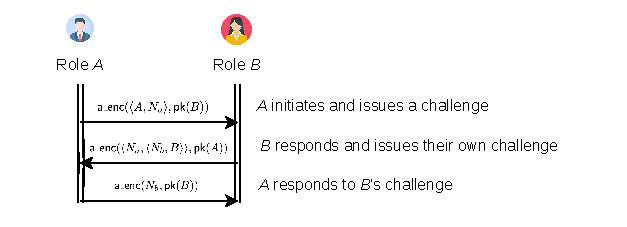
\includegraphics{figs/ns_type_confusion.pdf}
    \begin{flushleft}\footnotesize 
      Update to the original (flawed) Needham--Schroeder public-key protocol (Figure \ref{fig:ns-original}) 
      by replacing $\langle N_a, N_b \rangle$ with $\langle N_a, N_b, B \rangle^3$.
\end{flushleft}
  \caption{Update to Needham--Schroeder public-key protocol (in Figure \ref{fig:ns-original})} 
  \label{fig:ns-type-confusion}
\end{figure}

The only difference between this protocol and Figure \ref{fig:ns-original} is that in message $(2)$, we substituted $\langle N_a, \langle N_b, B \rangle \rangle$ for $\langle N_a, N_b \rangle$. Further, recall that we argued that using $\langle N_a, N_b, B \rangle^3$ (a triple, without nesting pairs) would make the protocol secure. While it is hard to believe at first glance, using the nested pairs $\langle N_a, \langle N_b, B \rangle \rangle$ rather than the triple is actually \textit{still insecure} in the symbolic model due to a type flaw attack.

Consider the following attack trace with intruder $I$, presented in Figure \ref{fig:type-confusion-attack}. 
In this trace, the capital letters 
$P_1$, $P_2$, and $I$ denote principals
(earlier, $A$ and $B$ denoted roles).

\begin{figure}[h!]
  \centering
  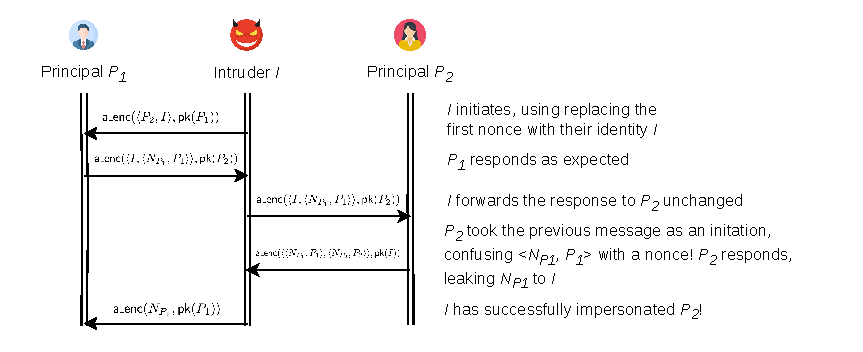
\includegraphics{figs/type_confusion_attack.pdf}
  \caption{Type confusion attack on Updated Needham--Schroeder public-key protocol (shown in Figure \ref{fig:ns-type-confusion})}
  \label{fig:type-confusion-attack}
\end{figure}

The ``type confusion" aspect of the attack is exhibited in step $3$ of the execution 
(Figure \ref{fig:type-confusion-attack})---$P_2$  
was expecting a message with format matching step $1$ (from Figure \ref{fig:ns-type-confusion}), 
but instead got one of format matching step $2$ (Figure \ref{fig:ns-type-confusion}). 
The attack works because $P_1$ does not destruct the pair in the protocol---if so, 
the incoming message would not unify with $P_1$'s expected message format. 
This also explains why using the triple $\langle N_a, N_b, B \rangle^3$ is not vulnerable to the same attack.

Type confusion attacks are somewhat controversial, and for good reason. One common argument in favor of design-level verification is that if there is a design-level vulnerability, then \emph{all} implementations will be affected. However, with type confusion attacks, this is not the case. One can imagine an implementation of the above protocol where role $B$ will not parse an input that substitutes a pair for a nonce, and hence the attack will not succeed. Hence, one may simply state \emph{a priori} that only well-typed attacks will be considered---this is called the \emph{strong typing assumption}.

\subsection{Typing protocols for free}\label{sec:typing}

In general, the strong typing assumption is not proof sound---a proof relying on the strong typing assumption may miss an attack (one that violates the assumption). However, for a certain class of protocols, the strong typing assumption \emph{is} proof sound---if there exists some type confusion attack, there must also exist another attack that does not rely on type confusion. In these cases, one may say we can ``type the protocol for free." To understand this claim more precisely, we must first concretize the idea of typing and ``well-typed attacks." 

\textbf{Tagging.} First, we take a quick detour to note that a straightforward \emph{tagging scheme} 
prevents type confusion attacks (more precisely, if a type confusion attack exists, then a well-typed attack exists). 
In this tagging scheme, we update each term in the protocol description $\mathsf{f}(t_1, \dots, t_n)$ 
to $\mathsf{f}(\langle \texttt{tag}_i, t_1 \rangle, \dots, t_n)$, 
each with a distinct  $\texttt{tag}_i$ (a concrete constant), 
and we update parsing to accommodate for the pair and require that honest participants check the tags 
to see that they match the expected values. 
The result (that tagging prevents type confusion) is formally proven in \cite{tagging}. 
It is not a trivial result, as the attacker may modify tags if they are not cryptographically protected.
%!! Indeed, modifying tags that are not cryptographically protected is 
% \emph{never necessary} to mount an attack under this tagging scheme.
% Intuitively, consider an attack trace that relies on modifying tags of some honest input term $t$
% to principal $A$. 
% Either $A$ attempts to destruct the term, or $A$ does not. 
% If so, then the tag modifications will be detected (as destruction will fail), 
% and the attack will fail. 
% If $A$ does not attempt to destruct the term, 
% then the only way for the tag modifications
% to have any relevance is if $A$ forwards $t$ to some other principal for processing. 
% If $A$ encrypts $t$, then the tagging scheme prevents any type confusion to begin with. 
% But if not, then the attacker could just as well have injected $t$ 
% \emph{this} point, without the type confusion!
% Intuitively, one can argue that only cryptographically protected subterms need to be tagged: for example, assume there is a type confusion attack where participant $A$ expects to receive (and forward) a non-encrypted atomic message, but instead receives (and forwards to $B$) a pair, which $B$ misinterprets as some other protocol message and destructs. This is the beginning of a type confusion attack---however, since the messages are unencrypted, the adversary can perform an analogous attack \emph{without} type confusion by simply injecting the pair to $B$ directly.
% In general, unencrypted terms are already subject to adversarial modification without needing type confusion. {what if pair is signed or something then can't be injected?}

\textbf{Typing systems.} A \textit{typing system} is a pair $(T, \delta)$ such that $T$ is a set of types and $\delta$ is a mapping from $\mathcal{T}(\Sigma_c, D)$ to $T$. A \textit{well-typed substitution} $\sigma$ preserves types---that is, $\delta(v) = \delta(v\sigma)$ for all $v \in V$. We call a typing system \emph{well-formed} if $(1)$ well-typed substitutions preserve types for every term $t$, i.e., $\delta(t) = \delta(t\sigma)$, and $(2)$ if $\delta(t) = \delta(t')$, then $mgu(t, t')$ is well-typed (for all terms $t$, $t'$). A protocol trace is called \emph{well-typed} if all the active substitutions constitute a well-typed substitution.

\textbf{Example typing system.} 
Consider an example typing system that captures term structure with a given set of atomic types 
$T_{\mathsf{atomic}} \subseteq T$. 
For example, we want the type of $\mathsf{f}(a, \mathsf{g}(b, c))$ to be 
$\mathsf{f}_\tau(\tau_a, \mathsf{g}_\tau(\tau_b, \tau_c))$, where the $\tau_i$s are not necessarily 
distinct and each $\tau_i$ represents the atomic type of data item $i$. 
Further, we use $\mathsf{f}_\tau$ to denote the type constructor associated with constructor \textsf{f}. 
We define $\delta$ as follows: 
\[
\delta(t) =
\begin{cases}
\mathsf{f}_\tau(\delta(t_1), \dots, \delta(t_n))
  & \textsf{if } t = \mathsf{f}(t_1, \dots, t_n), \\[4pt]
\text{some }\tau \in T_{\mathsf{atomic}} 
  & \textsf{if } t \text{ is some } v \in V.
\end{cases}
\]

\textbf{Type compliance.} The \textit{type compliance} requirement intuitively requires 
that all unifiable encrypted subterms in the protocol description have the same type. 
Informally, this requirement is similar in spirit to tagging---just 
as tagging makes distinct messages non-unifiable, 
type compliance makes encrypted terms of different types non-unifiable. 
To state this formally, we need the notion of \textit{transparent} constructor symbols, 
which intuitively can be freely destructed and constructed by the adversary. 
More formally, a constructor symbol \textsf{f} is \emph{transparent} if there exists a term 
$\mathsf{f}(t_1, \dots, t_n) \in \mathcal{T}(\Sigma, \{\square\})$ (denoting holes at data items) 
such that for any term $t \in \mathcal{T}(\Sigma, D)$ with top-level constructor symbol $\textsf{f}$, 
we have $\mathsf{f}(t_1, \dots, t_n)\{t \mapsto \square\}$ normalizes to $t$. 
By ``normalizes", we refer to normalization with respect to application 
of the destructor rules viewed as term rewriting rules, and hence we must have destructors 
that correspond to a convergent rewrite system. For example, pairing is transparent, 
witnessed by the term $\langle \pi_1(\square), \pi_2(\square) \rangle$. 
Notice that for any pair $p$ we insert into the holes, destructing and constructing 
(with $\pi_1, \pi_2$, and $\langle .,. \rangle$) always yields $p$. 
From transparent constructor symbols, we define the set of \emph{encrypted subterms} 
of a term $t$ as those subterms of $t$ whose top-level constructor symbol is not transparent. 
A configuration $(\mathcal{P}, \phi, \sigma)$ is \emph{type compliant} with respect 
to a well-formed typing system $(T, \delta)$ if, for all encrypted subterms $t, t'$ in $\mathcal{P}$ 
(in channel outputs or equality tests), the image of $\phi$, or the image of $\sigma$, 
then we have that there exists some substitution $\theta$ such that $t \theta = t'\theta$ 
implies $\delta(t) = \delta(t')$ (i.e., unifiable subterms have the same type). 
An execution $\mathcal{K} \xrightarrow{\pi:\;\mathsf{tr}} (\mathcal{P}, \phi, \sigma)$ 
is \emph{well-typed} if $\sigma$ is a well-typed substitution. 
The notation $\overline{\mathit{tr}}$ denotes the trace skeleton obtained from $\mathsf{tr}$ 
by replacing each $\mathsf{in}(c, R)$ with $\mathsf{in}(c, \square)$ and each $\mathsf{out}(c, w)$ 
with $\mathsf{out}(c, \square)$.

\begin{theorem}
Assume $\mathcal{D}$ is a convergent rewriting system and $(T, \delta)$ is a well-formed typing system. 
Further, assume configuration $\mathcal{K}$ is type compliant with respect to $(T, \delta)$ and $\mathcal{D}$.
If $\mathcal{K}\xrightarrow{\pi:\; \mathsf{tr}} \mathcal{K}'$ for some trace $\mathsf{tr}$ and configuration $\mathcal{K}'$, then there exists trace $\mathsf{tr}'$ such that $\mathcal{K}\xrightarrow{\pi:\; \mathsf{tr}'} \mathcal{K}'$, $\mathsf{tr}'$ is well-typed, and $\overline{\mathsf{tr}} = \overline{\mathsf{tr}'}$.
\end{theorem}
% {Details for the above---executions, barb equivalent and why it's good. For reachability we can phrase it in terms of reaching a barb. From paper, ``For example, secrecy of a data $s$ can easily be encoded by adding
% a witness process of the form $in(c,v).if\; v = s\; then\; out(secret\_violated,s)$." Double check this though, they don't use the ite.}

\subsection{Metatheorems of Symbolic Model Formalisms}
The symbolic model security protocol verification problem is undecidable \cite{undecidable1,undecidable2}. Cutting ill-typed traces out of the search space (as discussed in Section \ref{sec:typing}) is one means to heuristically cope with undecidability, but there are many more---too many to cover in depth. The various attempts are summarized in Table \ref{tab:metatheorems}.

The first group (in blue) denotes approaches that \emph{sacrifice completeness} for decidability. These works consider a bounded variant of the verification problem (bounding sessions, message sizes, or data items), and hence they can achieve decidability on the \emph{bounded} variant. Interestingly, while bounding sessions alone is enough to achieve decidability \cite{bounded_sessions}, bounding message (term) depth or the size of $\mathcal{D}$ (i.e., the number of fresh nonces) \emph{alone} still yields undecidability \cite{bounded_undecidable}.

The second group (in green) \emph{syntactically restricts protocols} to achieve decidability. For example, ping-pong protocols \cite{pingpong} intuitively require that a message be  passed back and forth (``ping-ponged"), where each subsequent message must be derived purely from cryptographic operations and the previous message without introducing extra data (e.g., fresh nonces). Then, the decidability proofs take advantage of the extra structural requirements of the protocol to soundly bound the search space.

The third group (in orange) investigates ways to \emph{heuristically cut the search space} with no decidability guarantee (our discussion of well-typed attacks in Section \ref{sec:typing} falls in this group \cite{typing_for_free}), the problem is still undecidable. Even without decidability, these results can be useful to inform the development of verification tools that perform well in practice.

The fourth group (in purple) denotes approaches that \emph{sacrifice soundness} to achieve termination. These papers describe abstract interpretation-based approaches to over-approximate adversarial knowledge. Hence, the tools may raise spurious attacks, similarly to the ``secrecy by typing" approach \cite{f7,dystar}.

\definecolor{grouponeLight}{RGB}{222,235,247}
\definecolor{grouponeDark}{RGB}{158,202,225}
\definecolor{grouptwoLight}{RGB}{229,245,224}
\definecolor{grouptwoDark}{RGB}{161,217,155}
\definecolor{groupthreeLight}{RGB}{254,230,206}
\definecolor{groupthreeDark}{RGB}{253,174,107}
\definecolor{groupfourLight}{RGB}{239,237,245}
\definecolor{groupfourDark}{RGB}{188,189,220}

\begin{table}[h!]
\small
\centering
\begin{tabular}{|p{2cm}|p{1.6cm}p{2.6cm}p{2.6cm}p{1.7cm}p{2.6cm}|}
\hline
\textbf{Paper} &
\textbf{Formalism} &
\textbf{Restrictions} &
\textbf{Benefit} &
\textbf{Fragment decidable?} &
\textbf{Formal}\newline\textbf{guarantees} \newline (wrt unbounded) \\
\hline

\rowcolor{grouponeDark}
Rusinowitch \& Turuani \cite{bounded_sessions} & DY & bounded sessions & NP-completeness & yes & AS \\ 

\rowcolor{grouponeLight}
Durgin eg al. \cite{bounded_undecidable} & multiset rewriting & bound message size and $|\mathcal{D}|$ & EXPTIME-completeness & yes & AS \\

\rowcolor{grouponeDark}
Ramanujam \& Suresh \cite{tagged_bounded_secrecy} & DY & tagged protocols, bounded messages, secrecy properties & decidability & yes & AC, PC \\

\hhline{|======|}

\rowcolor{grouptwoDark}
Dolev et al. \cite{pingpong} & DY & ping-pong \cite{pingpong} protocols & PTIME-completeness & yes & AS, PS, AC, PC \\ 

\rowcolor{grouptwoLight}
Ramanujam \& Suresh \cite{context_explicit} & DY & context-explicit \cite{context_explicit} protocols, secrecy properties & NEXP-time & yes & AS, PS, AC, PC \\

\rowcolor{grouptwoDark}
D'Osualdo et al. \cite{depth_bounded} & applied $\pi$-calculus & depth-bounded protocols \cite{depth_bounded} & decidability & yes & AS, PS, AC, PC \\

\rowcolor{grouptwoLight}
Lowe \cite{small_model} & DY & context-explicit, inferrable identities, no temporary secrets, secrecy properties & small model theorem (one session with one principal per role) & yes & AS, PS, AC, PC \\

\hhline{|======|}

\rowcolor{groupthreeDark}
 Cortier et al. \cite{bound_sessions} & applied \newline $\pi$-calculus & Type compliance, simple protocols$^*$, no else branches$^*$  & heuristically soundly bound number of sessions & no & AS, PS \\

\rowcolor{groupthreeLight}
  Chrétien et al. \cite{typing_for_free} & applied \newline $\pi$-calculus & type compliance, convergent \newline equational theory & cut ill-typed \newline attacks from search space & no & PS, AS \\

\rowcolor{groupthreeDark}
   Lowe \& Schneider \cite{tagging} & strand spaces & tagged protocols & cut ill-typed \newline attacks from search space & no & PS, AS \\

\rowcolor{groupthreeLight}
   Blanchet \& Podelski \cite{tagging_enforces_termination} & applied $\pi$-calculus/ Horn clauses & tagged protocols & termination & no & PS \\


\hhline{|======|}

\rowcolor{groupfourDark}
Nielson et al. \cite{cubic_time} & DY & secrecy properties & termination (through approximation)  & yes & PS, AC \\

\rowcolor{groupfourLight}
Goubault-Larrecq \cite{ai_1} & DY & secrecy properties & termination (through approximation) & yes & PS, AC \\

\rowcolor{groupfourDark}
Heather \& Schneider \cite{ai_2} & CSP & auth properties  & termination (through approximation) & yes & PS, AC \\

 \hline


\end{tabular}
\begin{flushleft}
\vspace{0.3em}
DY is shorthand for any formalism that closely follows the original Dolev-Yao encoding 
\cite{dolev_yao}. It is very similar in spirit to strand spaces \cite{strand_spaces}, 
and can only encode simple (stateless, purely cryptographic) protocols.
\newline\newline
Blue (first group) denotes approaches \emph{sacrificing completeness for decidability}. Green (second group) denotes approaches \emph{syntactically restricting protocols for decidability}. Orange (third group) denotes approaches to \emph{heuristically cut the search space} (without a termination guarantee). Purple (fourth group) denotes approaches \emph{sacrificing soundness for termination}.
\newline\newline
$^*$Only needed for equivalence properties. 
\end{flushleft}

\caption{Symbolic model metatheorems}
\label{tab:metatheorems}
\end{table}



\section{Open Research Problems}\label{sec:open-questions}
In light of previous work on symbolic model verification, we now discuss some open research questions.
\begin{itemize}
    % \item Strengthening the threat model a la CCSA
    \item[\textsf{RQ1.}] 
    \textbf{How to reason about cryptographic protocols with heavy non-cryptographic aspects in a single formalism, 
    while also retaining some  automation.} 
    As discussed in the introduction, many protocols like 4G LTE/5G 
    (as well as the Uptane \cite{uptane} over-the-air software update protocol) 
    involve heavy non-cryptographic reasoning. 
    Prior work \cite{5greasoner,lteinspector,uptane_analysis} maintains some automation, 
    but it relies on two separate protocol models, 
    one in a standard CPV (like ProVerif or Tamarin) and another in a general-purpose model checker (like Kind 2 or nuXmv). 
    Ideally, reasoning could proceed with ``one model to rule them all." 
    Note that none of the tools in Table \ref{tab:tools} have robust, 
    dedicated theory reasoning, except for the third group (F7 and DY$^*$). 
    However, these tools raise spurious violations through their usage of manually-annotated security labels.  
    Additionally, one could achieve these goals with an ITP; however, this approach abandons automation.
    \item[\textsf{RQ2.}] 
    \textbf{How to reason about protocols with unbounded loops and recursive datatypes, 
    without resorting to manually annotated security labels (or more generally, spurious violations).} 
    Of the tools in Table \ref{tab:tools}, only Tamarin has \emph{partial} 
    support for protocols with loops (requiring expertise with non-standard modeling techniques 
    in Tamarin \cite{tamarin_looping}), and none natively support recursive datatypes, 
    save for the third group (F7 and DY$^*$). Again, one must either accept spurious violations 
    (from F7 or DY$^*$) or abandon automation (by using an ITP).
    \item[\textsf{RQ3.}] 
    \textbf{How to reason about cryptographic protocols compositionally.} 
    Besides the third group (F7 and DY$^*$), all of the tools in Table \ref{tab:tools} reason monolithically. 
    In the context of compositional verification, \emph{automatically inferring} a good decomposition is a very hard problem 
    in general, 
    and the combined cost of inferring decompositions and compositional reasoning may not be more efficient 
    than simply reasoning monolithically
    \cite{cobleigh1,cobleigh2}.
    There is prior work that investigates compositional reasoning in the context of separation logic \cite{generic_methodology}; 
    however, it suffers from the similar downsides as F7 and DY$^*$.
    While automatically inferring decompositions is difficult in general, 
    one might intuit that it could be feasible in the context of security protocols---lots of protocols 
    have ``similar" shapes with honest steps and an adversaries with similar sets of capabilities. 
    \item[\textsf{RQ4.}] \textbf{How to reason about the composition of cryptographic protocols.} 
    Consider two protocols $P_1$ and $P_2$, and assume that $P_1$ satisfies security property 
    $\varphi$ (i.e., $P_1 \models \varphi$). 
    What can one say about the asynchronous parallel composition of $P_1$ and $P_2$? 
    One cannot lift the results of the separate analyses to the composed case in any straightforward way 
    due to adversarial influence---the adversary may use information learned from some run of $P_2$ 
    to influence a run of $P_1$, possibly violating $\varphi$.
    \item[\textsf{RQ5.}] \textbf{How to recover useful interactivity when automated techniques fail to terminate or produce spurious violations.} 
    A weakness of all tools in Table \ref{tab:tools} is that when verification fails (through nontermination or spurious violations), 
    there is no effective means of isolating the problem. 
    Again, ITPs are strong here, but lack automation.
    Ideally, a tool would have high automation potential, but when the proof fails, 
    there would be a means of interaction that isolates a hole in the proof with unfinished local goals. 
\end{itemize}

\section{Conclusion}

Symbolic model cryptographic protocol verification has developed into a killer application 
for formal methods and automated reasoning, as it focuses on problems that are hard to get right but still tractable for 
(semi-)automated techniques. Multiset rewriting and applied $\pi$-calculus have been intensely studied to that end for many years, 
both in terms of theory and practical algorithms. 
However, there are fundamental obstacles to advancing symbolic model verification in these settings. 
One major obstacle is that these formalisms are inherently monolithic, which is in conflict with usable 
interactivity---for humans, it is easier to conceptualize decomposed problems. 
Further, while the existing algorithms work well for cryptographic operations, 
they do not generalize well for protocols heavy on non-cryptographic reasoning. 
To address these issues, the security community may be able to draw inspiration 
from existing approaches in the (general-purpose) verification community.

\bibliographystyle{plain}
\bibliography{biblio}
 
% \section{Questions}
% \begin{itemize}
%     % \item {Why does Horn clause representation of adversary knowledge overapproximation not lead to spurious secrecy counterexamples? Why can't we just pick a model where adv(x) holds?}
% \item In metatheorems, security problem vs secrecy problem? A: Secrecy is restricted/specific, security would be more like any property formalizable in Tamarin's language (or whoever's language)
% \item How can there be distinct MGUs? A: See example in slides of two solutions when you have XOR, you get two unifiers. I think they are incomparable?
% \item What part of unification algo + AC breaks if we don't have AC-coherence? A: AC-coherence is essentially another diamond property that becomes relevant with equational theories. Like it says "if s =_E t and s -->*_E t', then t -->*_E t'" or similar
% \item How is proverif's overapproximation of attacker-computable terms different from secrecy by typing world, e.g. DY$^*$? A: Overapprox has to do with protocol control flow, which is somewhat orthogonal to overapprox due to security labels and lack of ``smallest relation containing" semantics (which ProVerif gets from resolution algo)
% \item What are the 0-ary constants in the Herbrand universe of ProVerif's Horn clause representation? It seems like in the Horn clause translation, ``patterns" produce function symbols (including 0-arity)
% \item Why does the typing protocols for free paper require convergent destructor rules? Why can't we work with unnormalized terms? One part of it is that the definition of ``transparent" relies on normal forms, but this seems like it could be worked around.
% \item Where are the structural equivalence rules in ``typing protocols for free"? A: Captured in ``Par" and semantics of multisets
% \end{itemize}

\end{document}

